\section{2. Comparing the Read Data. } 

\subsection{1. What concern about are...}
\begin{frame}[c,fragile]
	\begin{block}{ Difference in regions: }
		\begin{itemize}
			\item Gene regions.
			\begin{itemize}
				\item Difference FPKM (cufflinks)? \\
				\item Difference Read Counts (Hiseq)? \\
			\end{itemize}
			\item Repeat regions.
			\begin{itemize}
				\item Difference FPKM (cufflinks)? \\
				\item Difference Read Counts (Hiseq)? \\
			\end{itemize}
		\end{itemize}
	\end{block}
\end{frame}


\subsection{2.Reads mapped to gene-region.}

\begin{frame}[c,fragile]
	\frametitle{ For refseq genes, TT $>$ HT $\approx$ HM $>$ TM. }
		\tiny{
			\begin{table}
			\centering
			\begin{tabular}{  C{0.4cm}  C{1.3cm}  C{1.3cm}  C{1.3cm}  C{1.3cm} C{1.0cm} C{0.75cm} C{0.75cm} }
			\hline\noalign{\smallskip}
			Samp & Pre & Aln & Known & Rfseq & Non4 & Nsmb & Neo \\
			\noalign{\smallskip}\hline\noalign{\smallskip}			
			TT &	217,499K & 181,322K & 172,295K & 170,471K & 1,816K & 7604 & 34486	 \\
			TM &	217,499K & 177,886K & 157,031K & 153,429K & 3,593K & 8000 & 214952  \\
			HT &	217,499K & 195,486K & 165,746K & 163,356K & 2,382K & 8236 & 65284	 \\
			HM &	217,499K & 195,455K & 165,575K & 163,186K & 2,380K & 8238 & 65506	 \\
			\noalign{\smallskip}\hline  		\\
			\end{tabular}
			\end{table}
		}
	
\end{frame}


\begin{frame}[c,fragile]
	\frametitle{ Result calculated by cuffquant-cuffnorm. }
	\begin{block}{ FPKM for genes. }
			\begin{table}
			\centering	
			\begin{tabular}{C{4cm}  C{4cm}}     
				Transcripts in genome		& ERCC spike-ins 	\\
				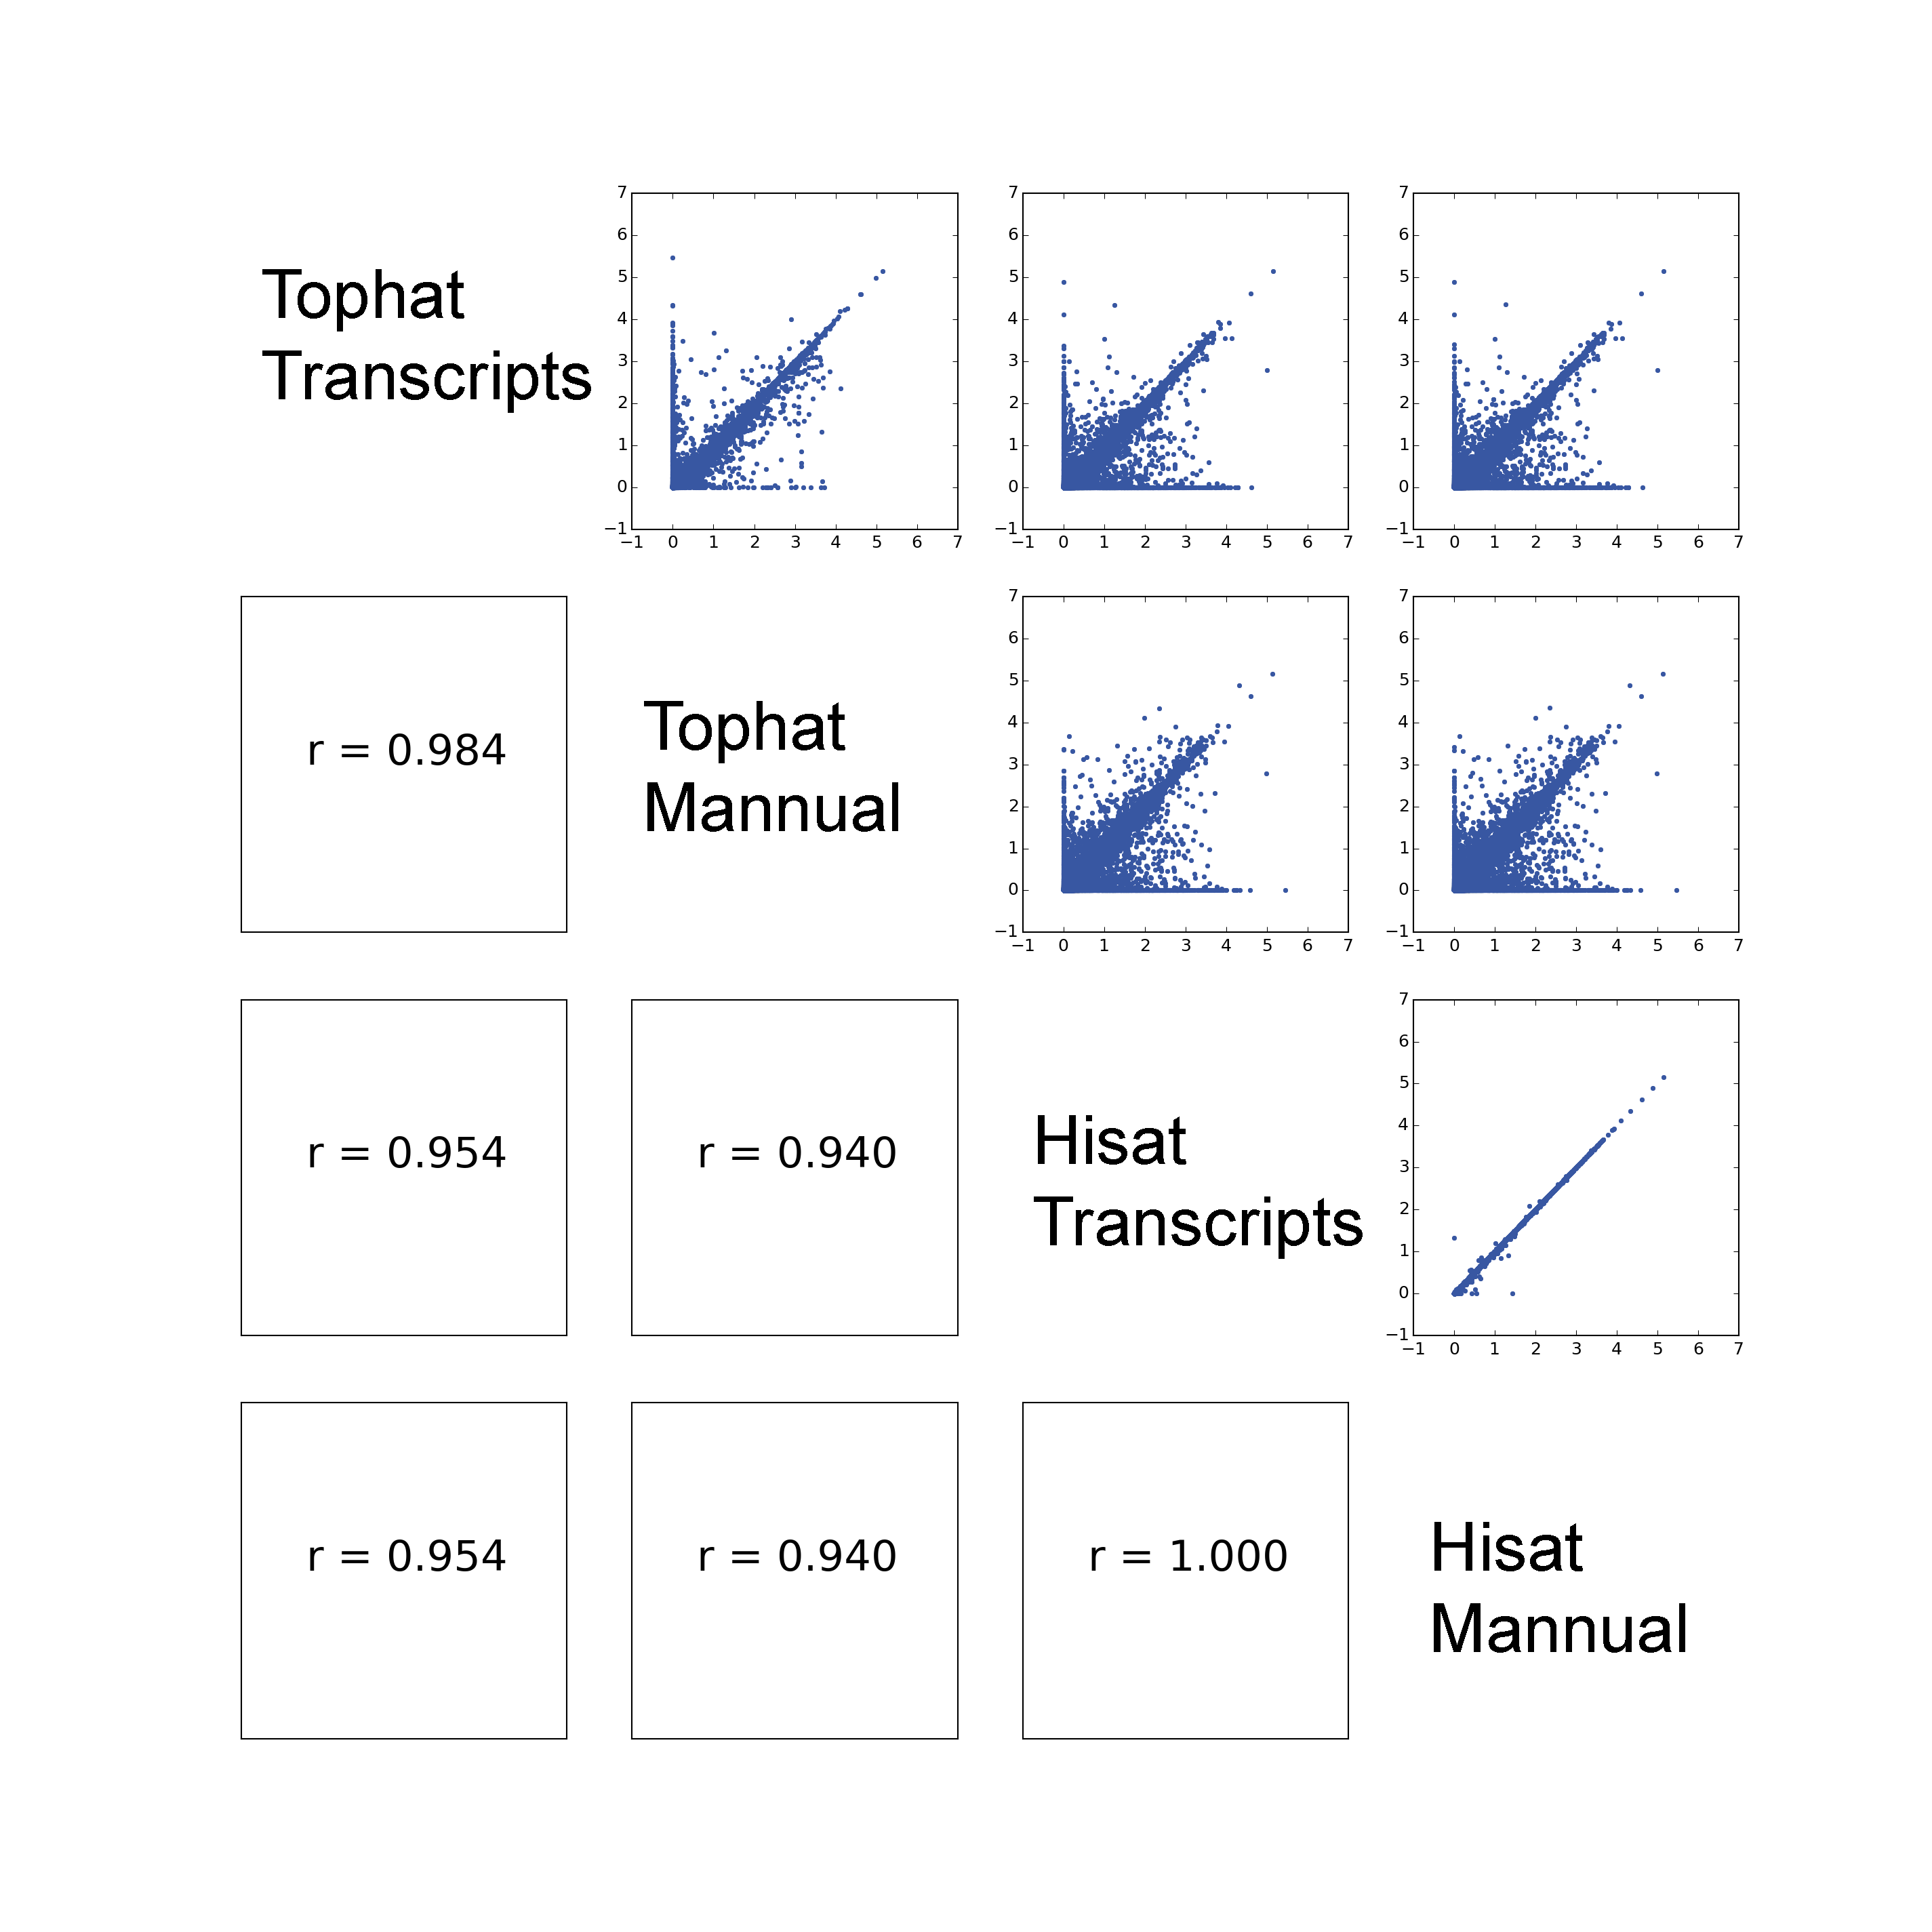
\includegraphics[height=4cm]{All_FPKM}	&  
				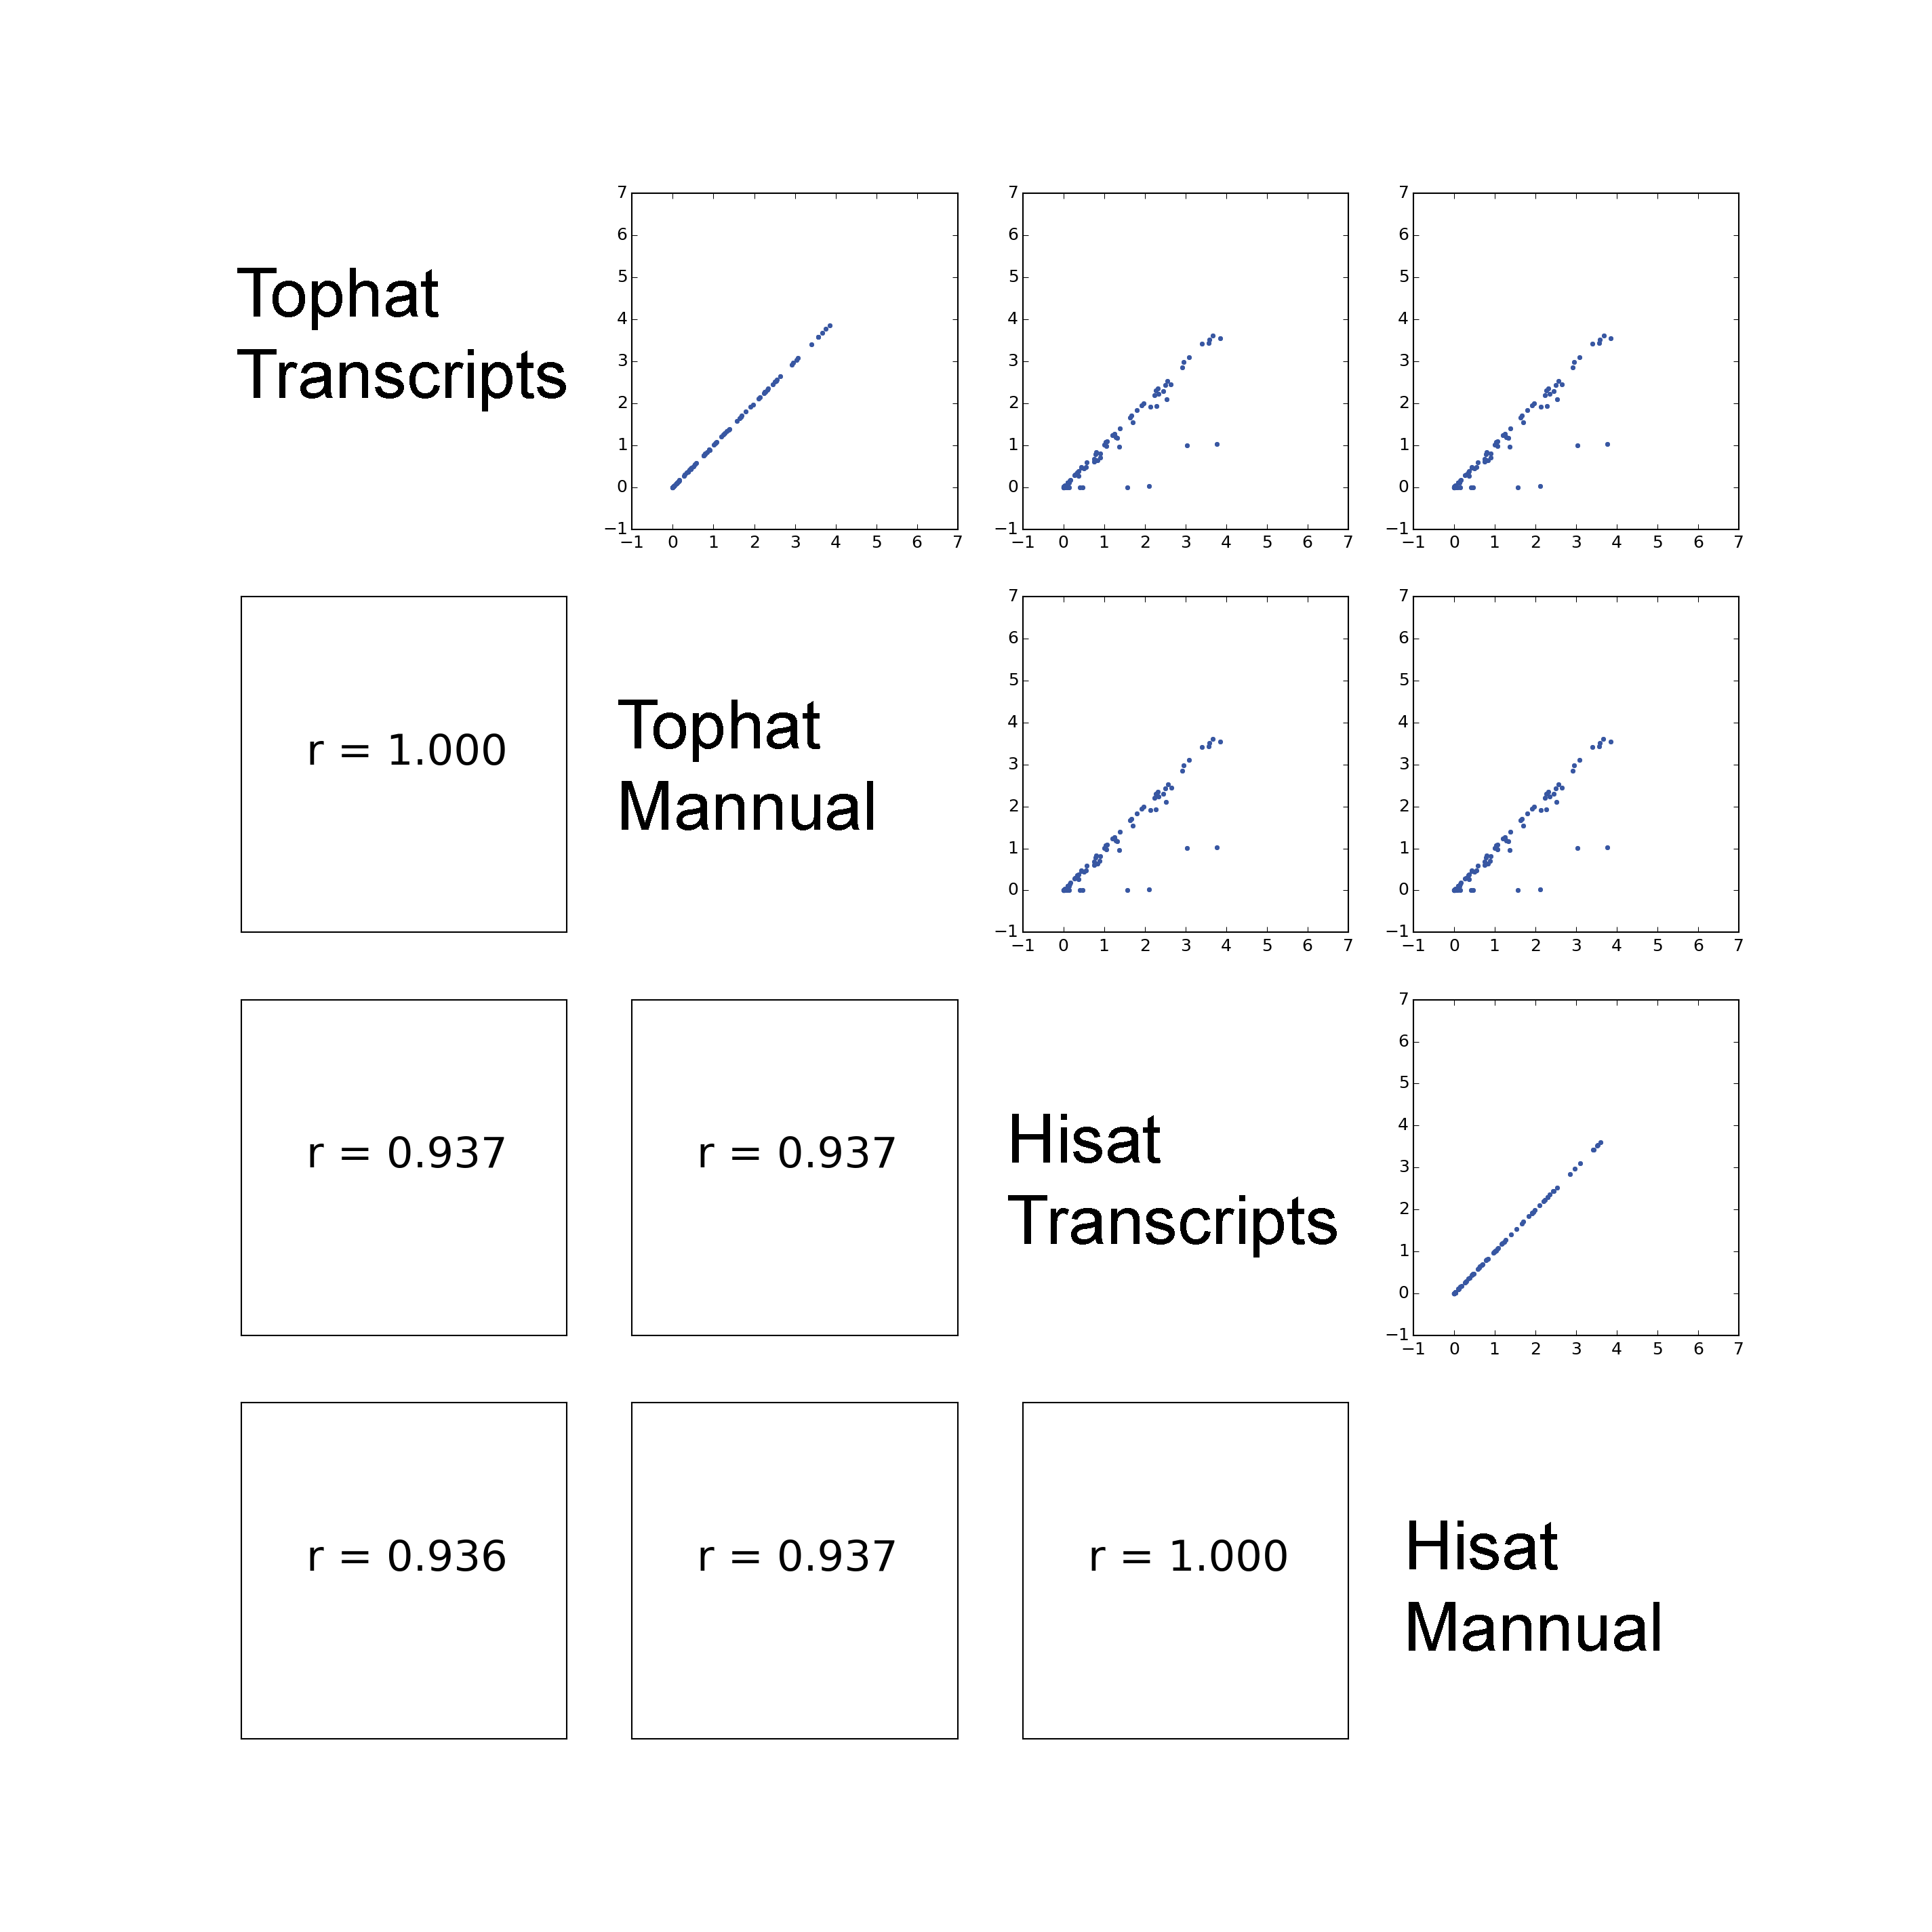
\includegraphics[height=4cm]{ERCC_FPKM}	\\	
			\end{tabular}	
			\end{table}	
			Higher for ERCC using Hisat.
	\end{block}
\end{frame}

\begin{frame}[c,fragile]
	\frametitle{ Result calculated by cuffquant-cuffnorm. }
	\begin{block}{ FPKM for Refseq genes and Noncode v4 transcripts. }
			\begin{table}
			\centering	
			\begin{tabular}{C{4cm}  C{4cm}}     
				Refseq genes		& Noncode v4 	\\
				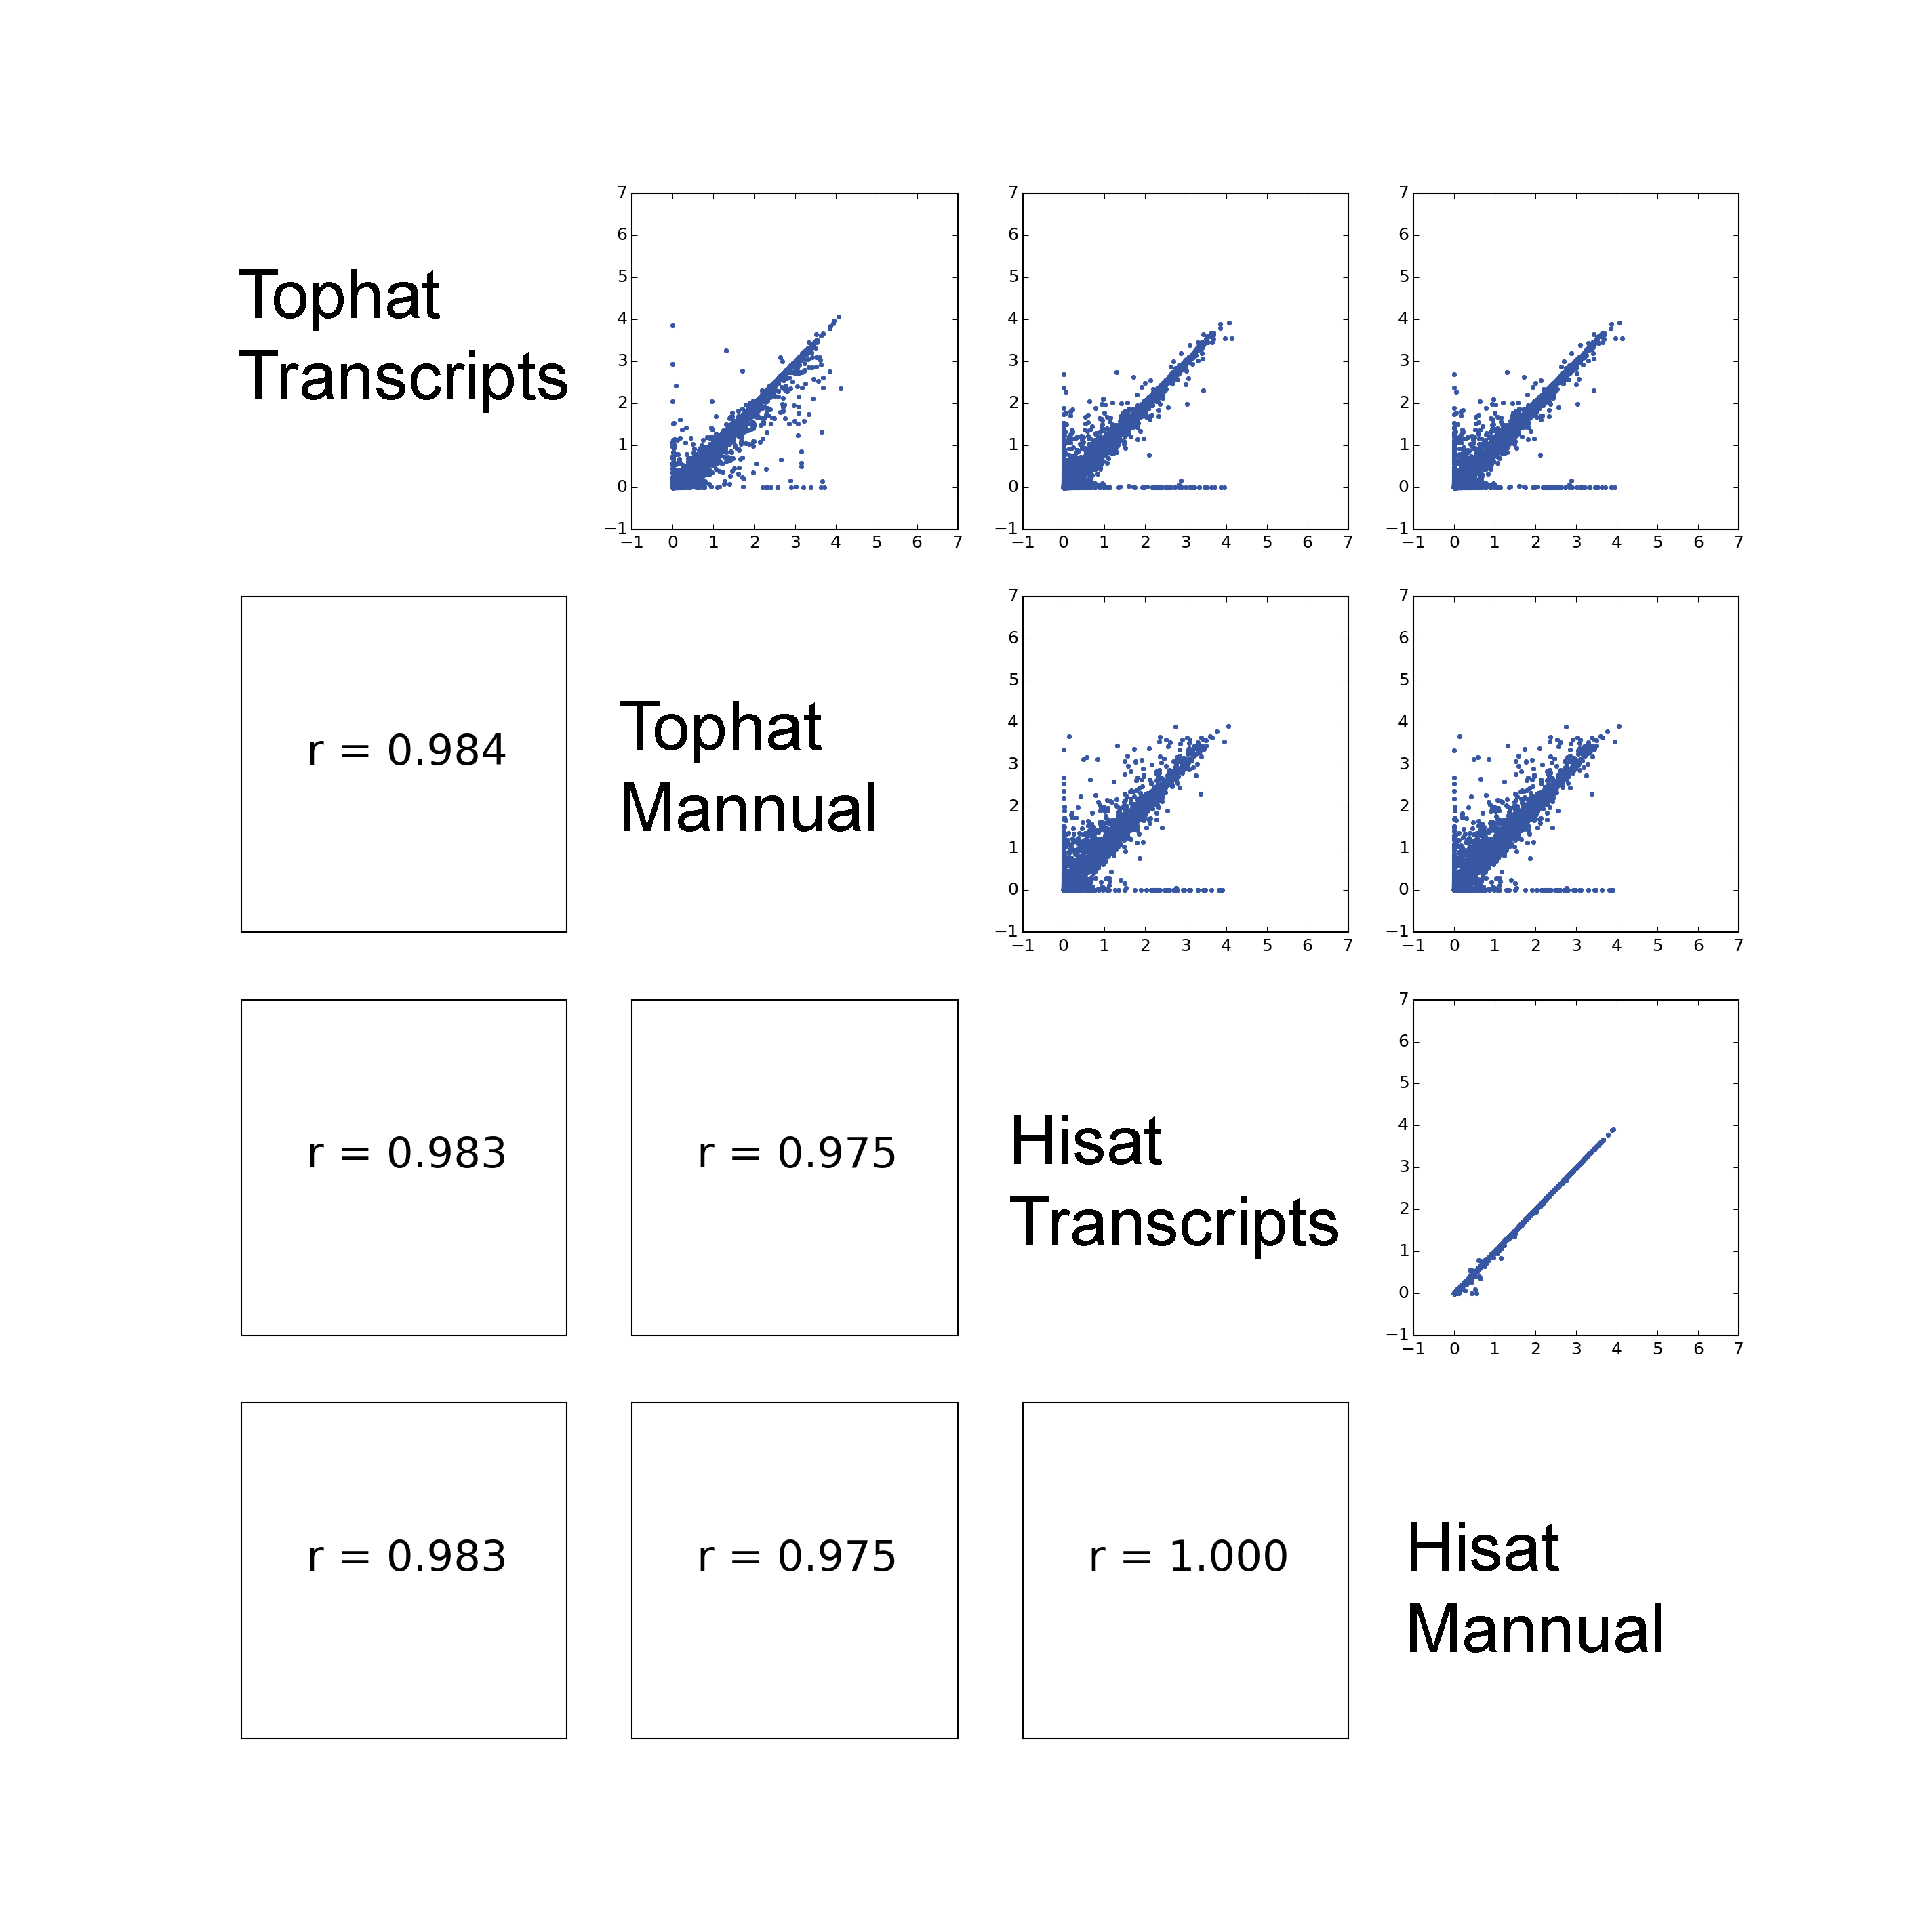
\includegraphics[height=4cm]{Refgene_FPKM}	&  
				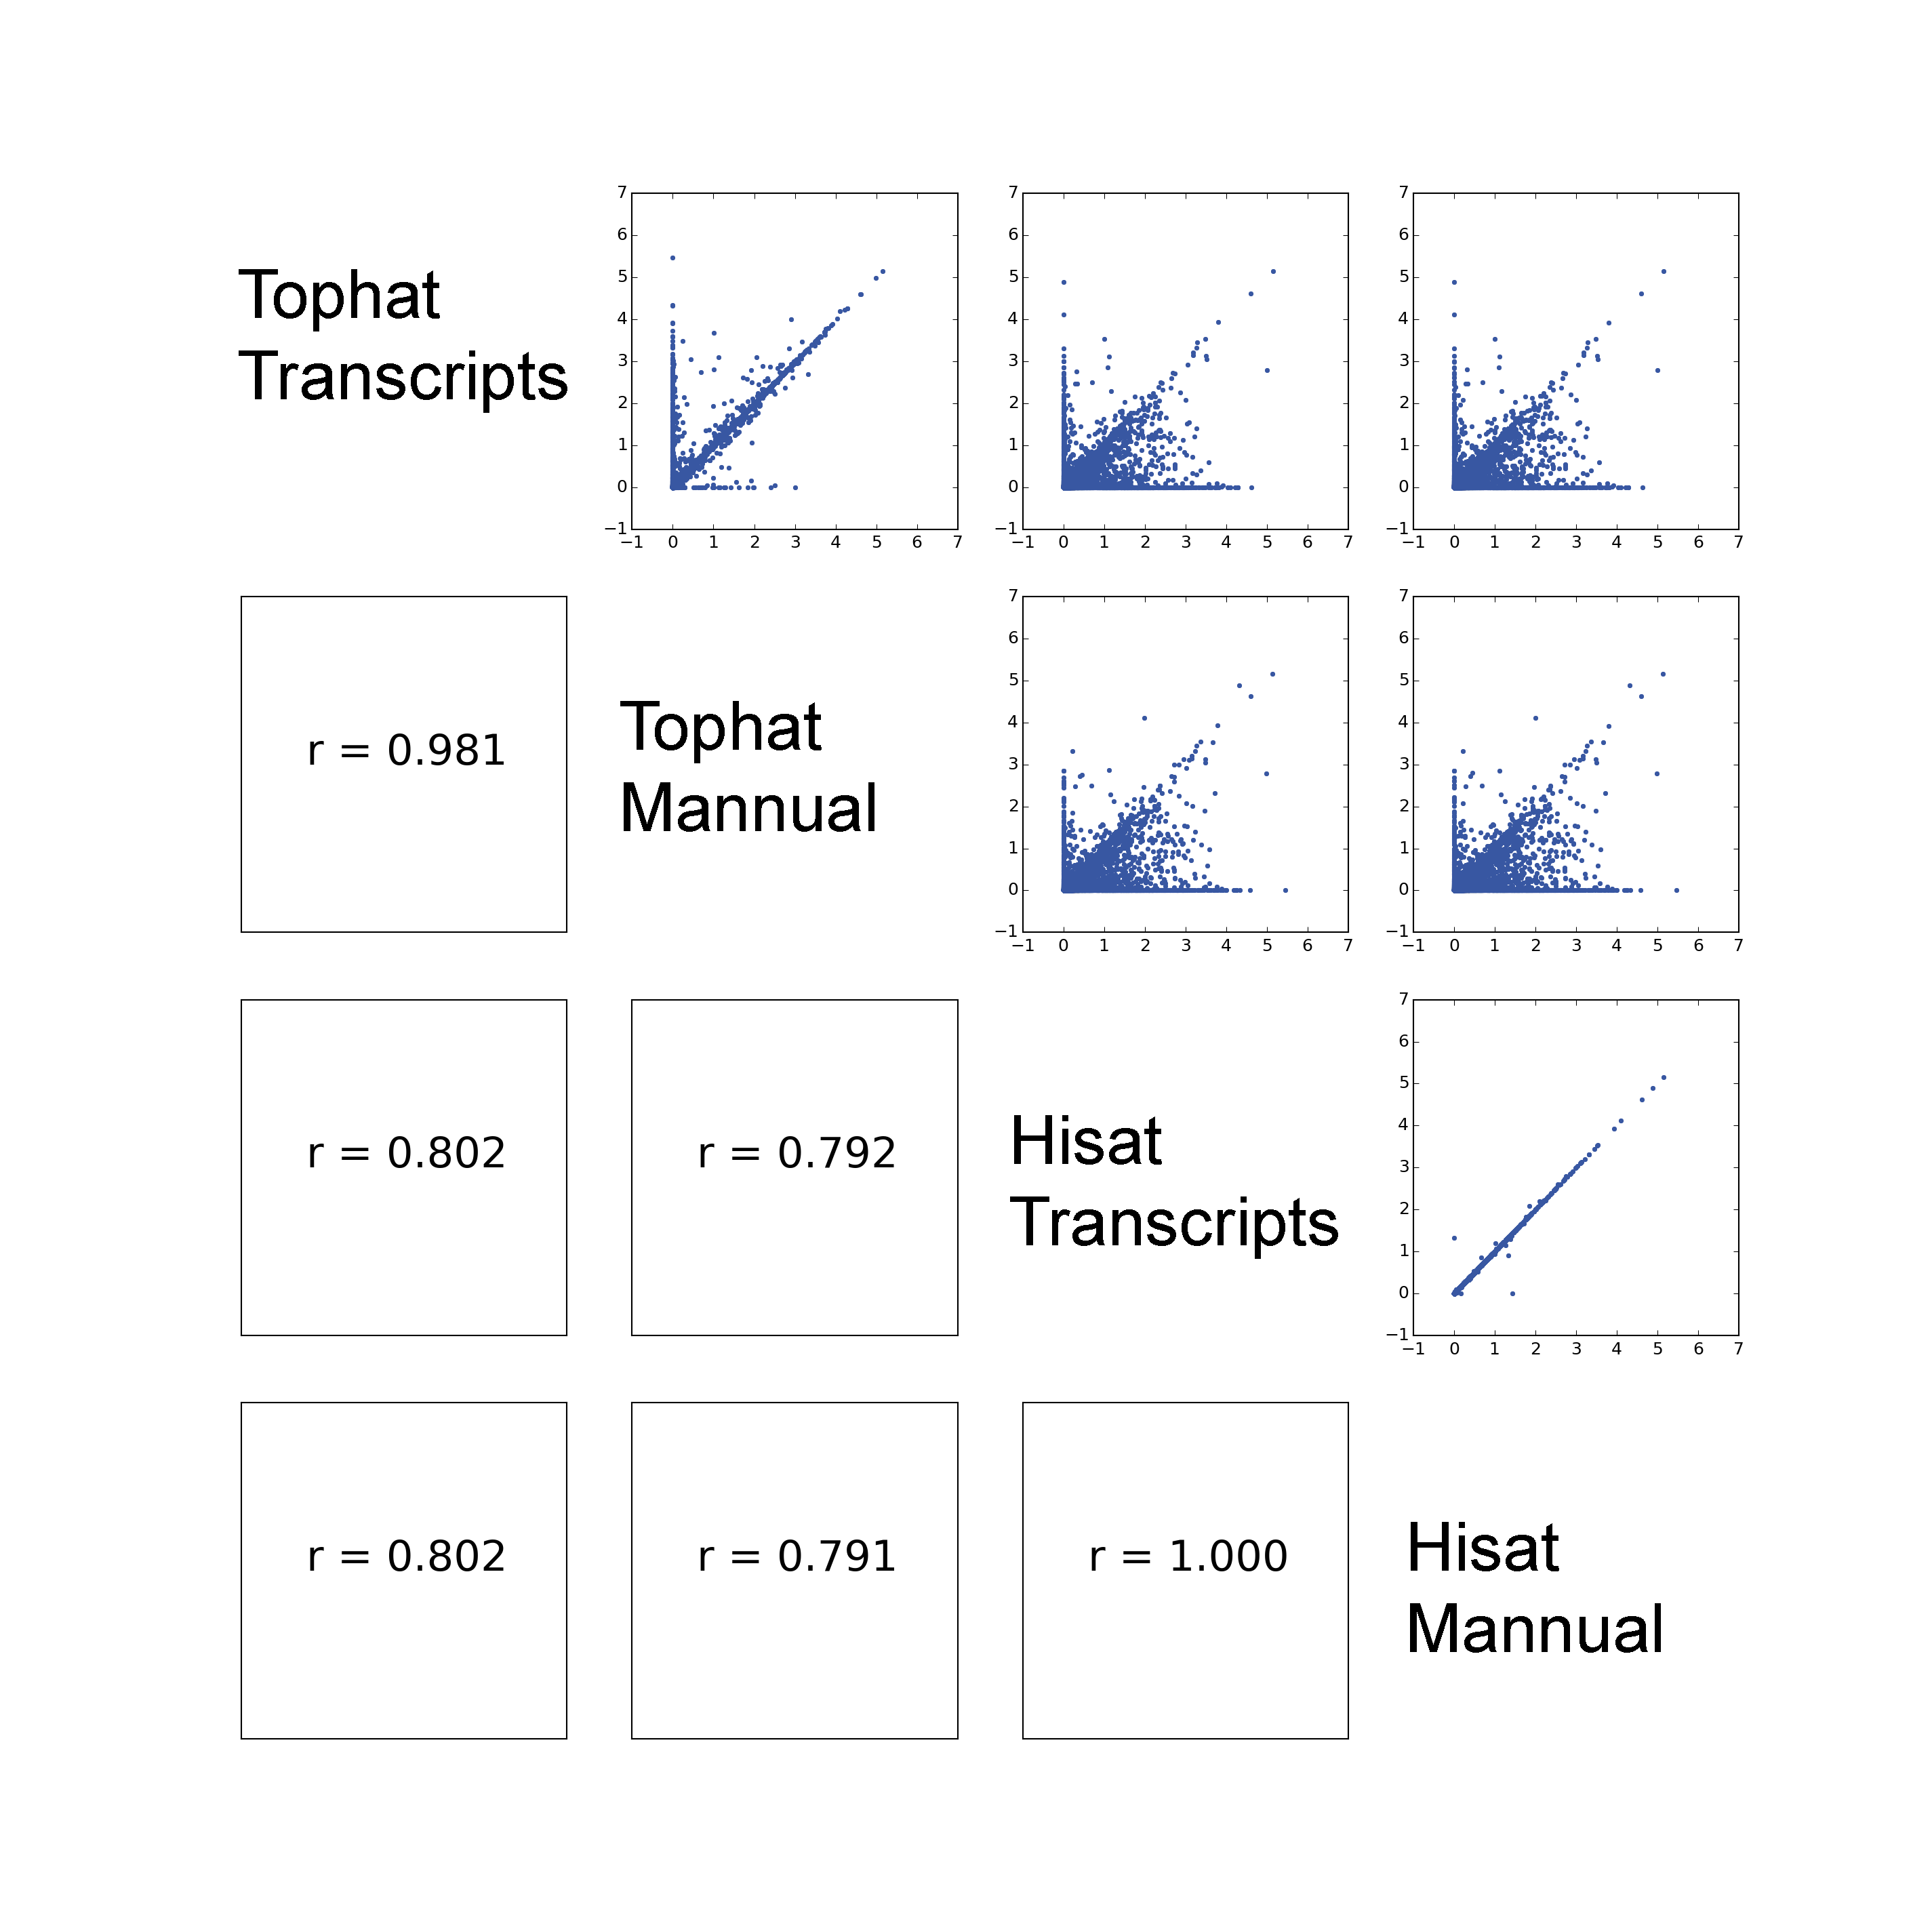
\includegraphics[height=4cm]{NONCODE_FPKM}	\\	
			\end{tabular}	
			\end{table}	
	\end{block}
\end{frame}

\begin{frame}[c,fragile]
	\frametitle{ Refseq: (((HT,HM),TM),TT); ERCC: almost the same. }
	\begin{block}{ Read Counts for refseq-genes. }
			\begin{table}
			\centering	
			\begin{tabular}{C{4cm}  C{4cm}}     
				Refseq genes		& ERCC spike-ins 	\\
				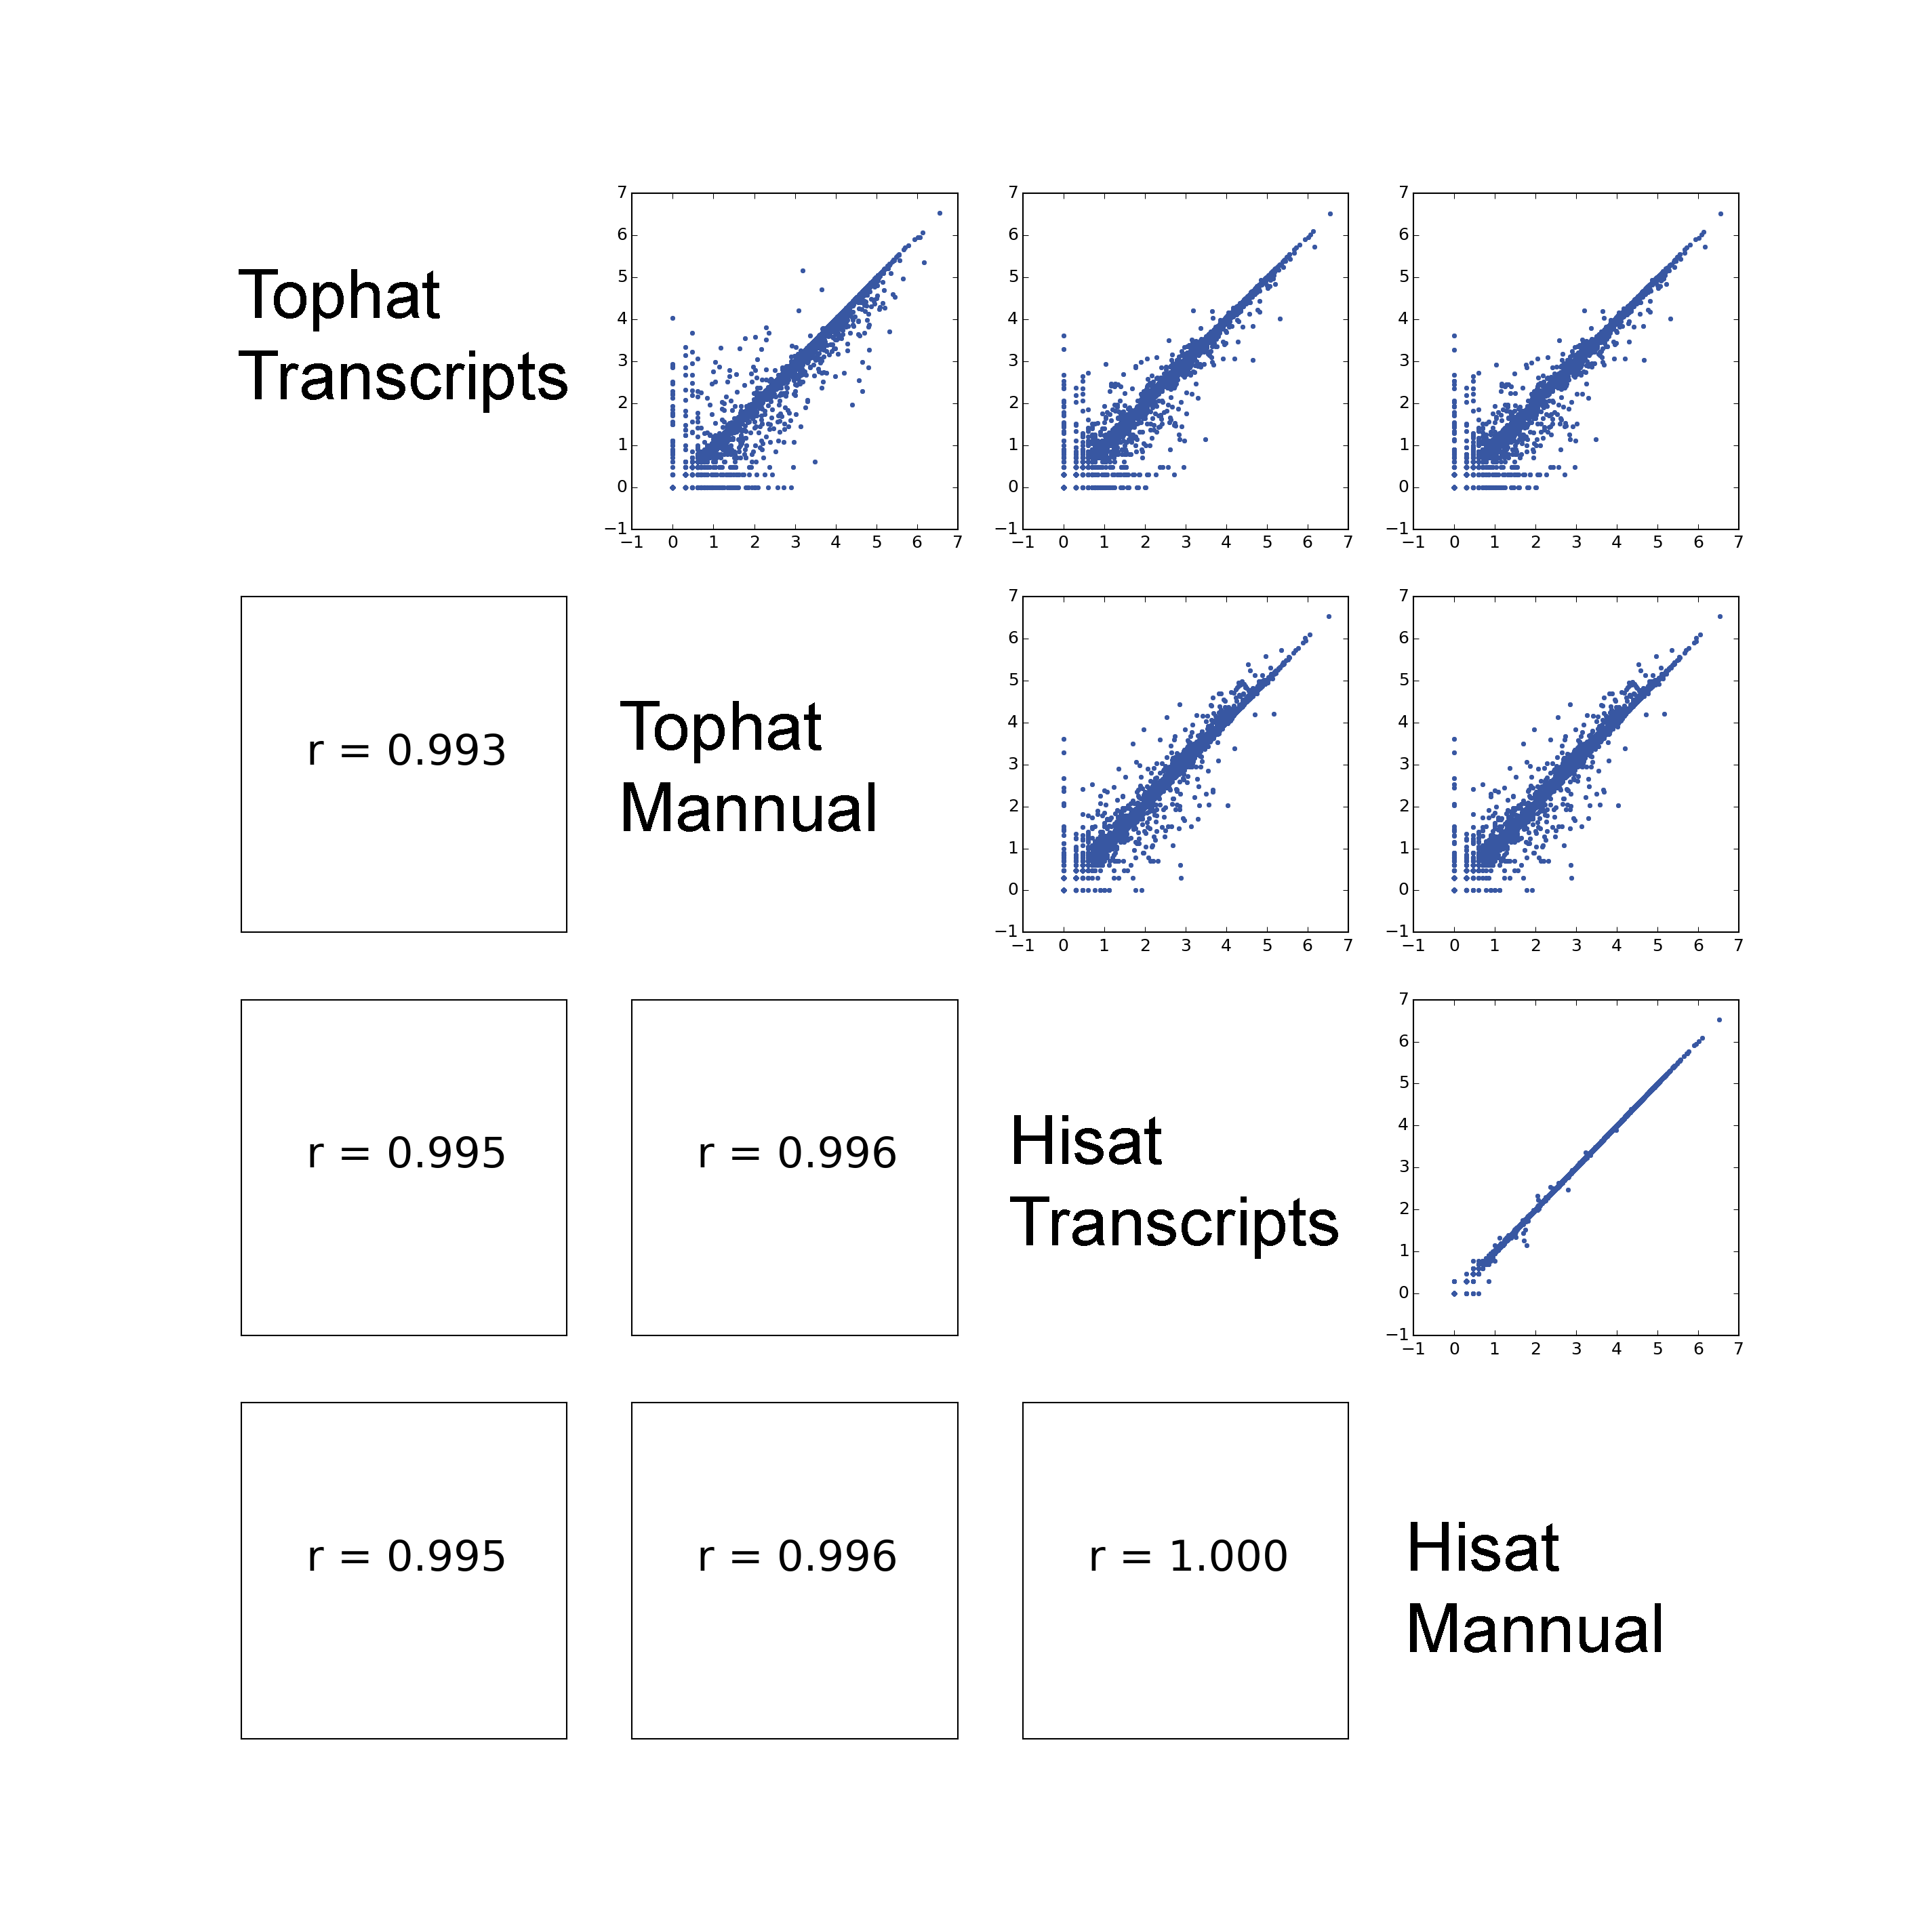
\includegraphics[height=4cm]{Refseq_count}	&  
				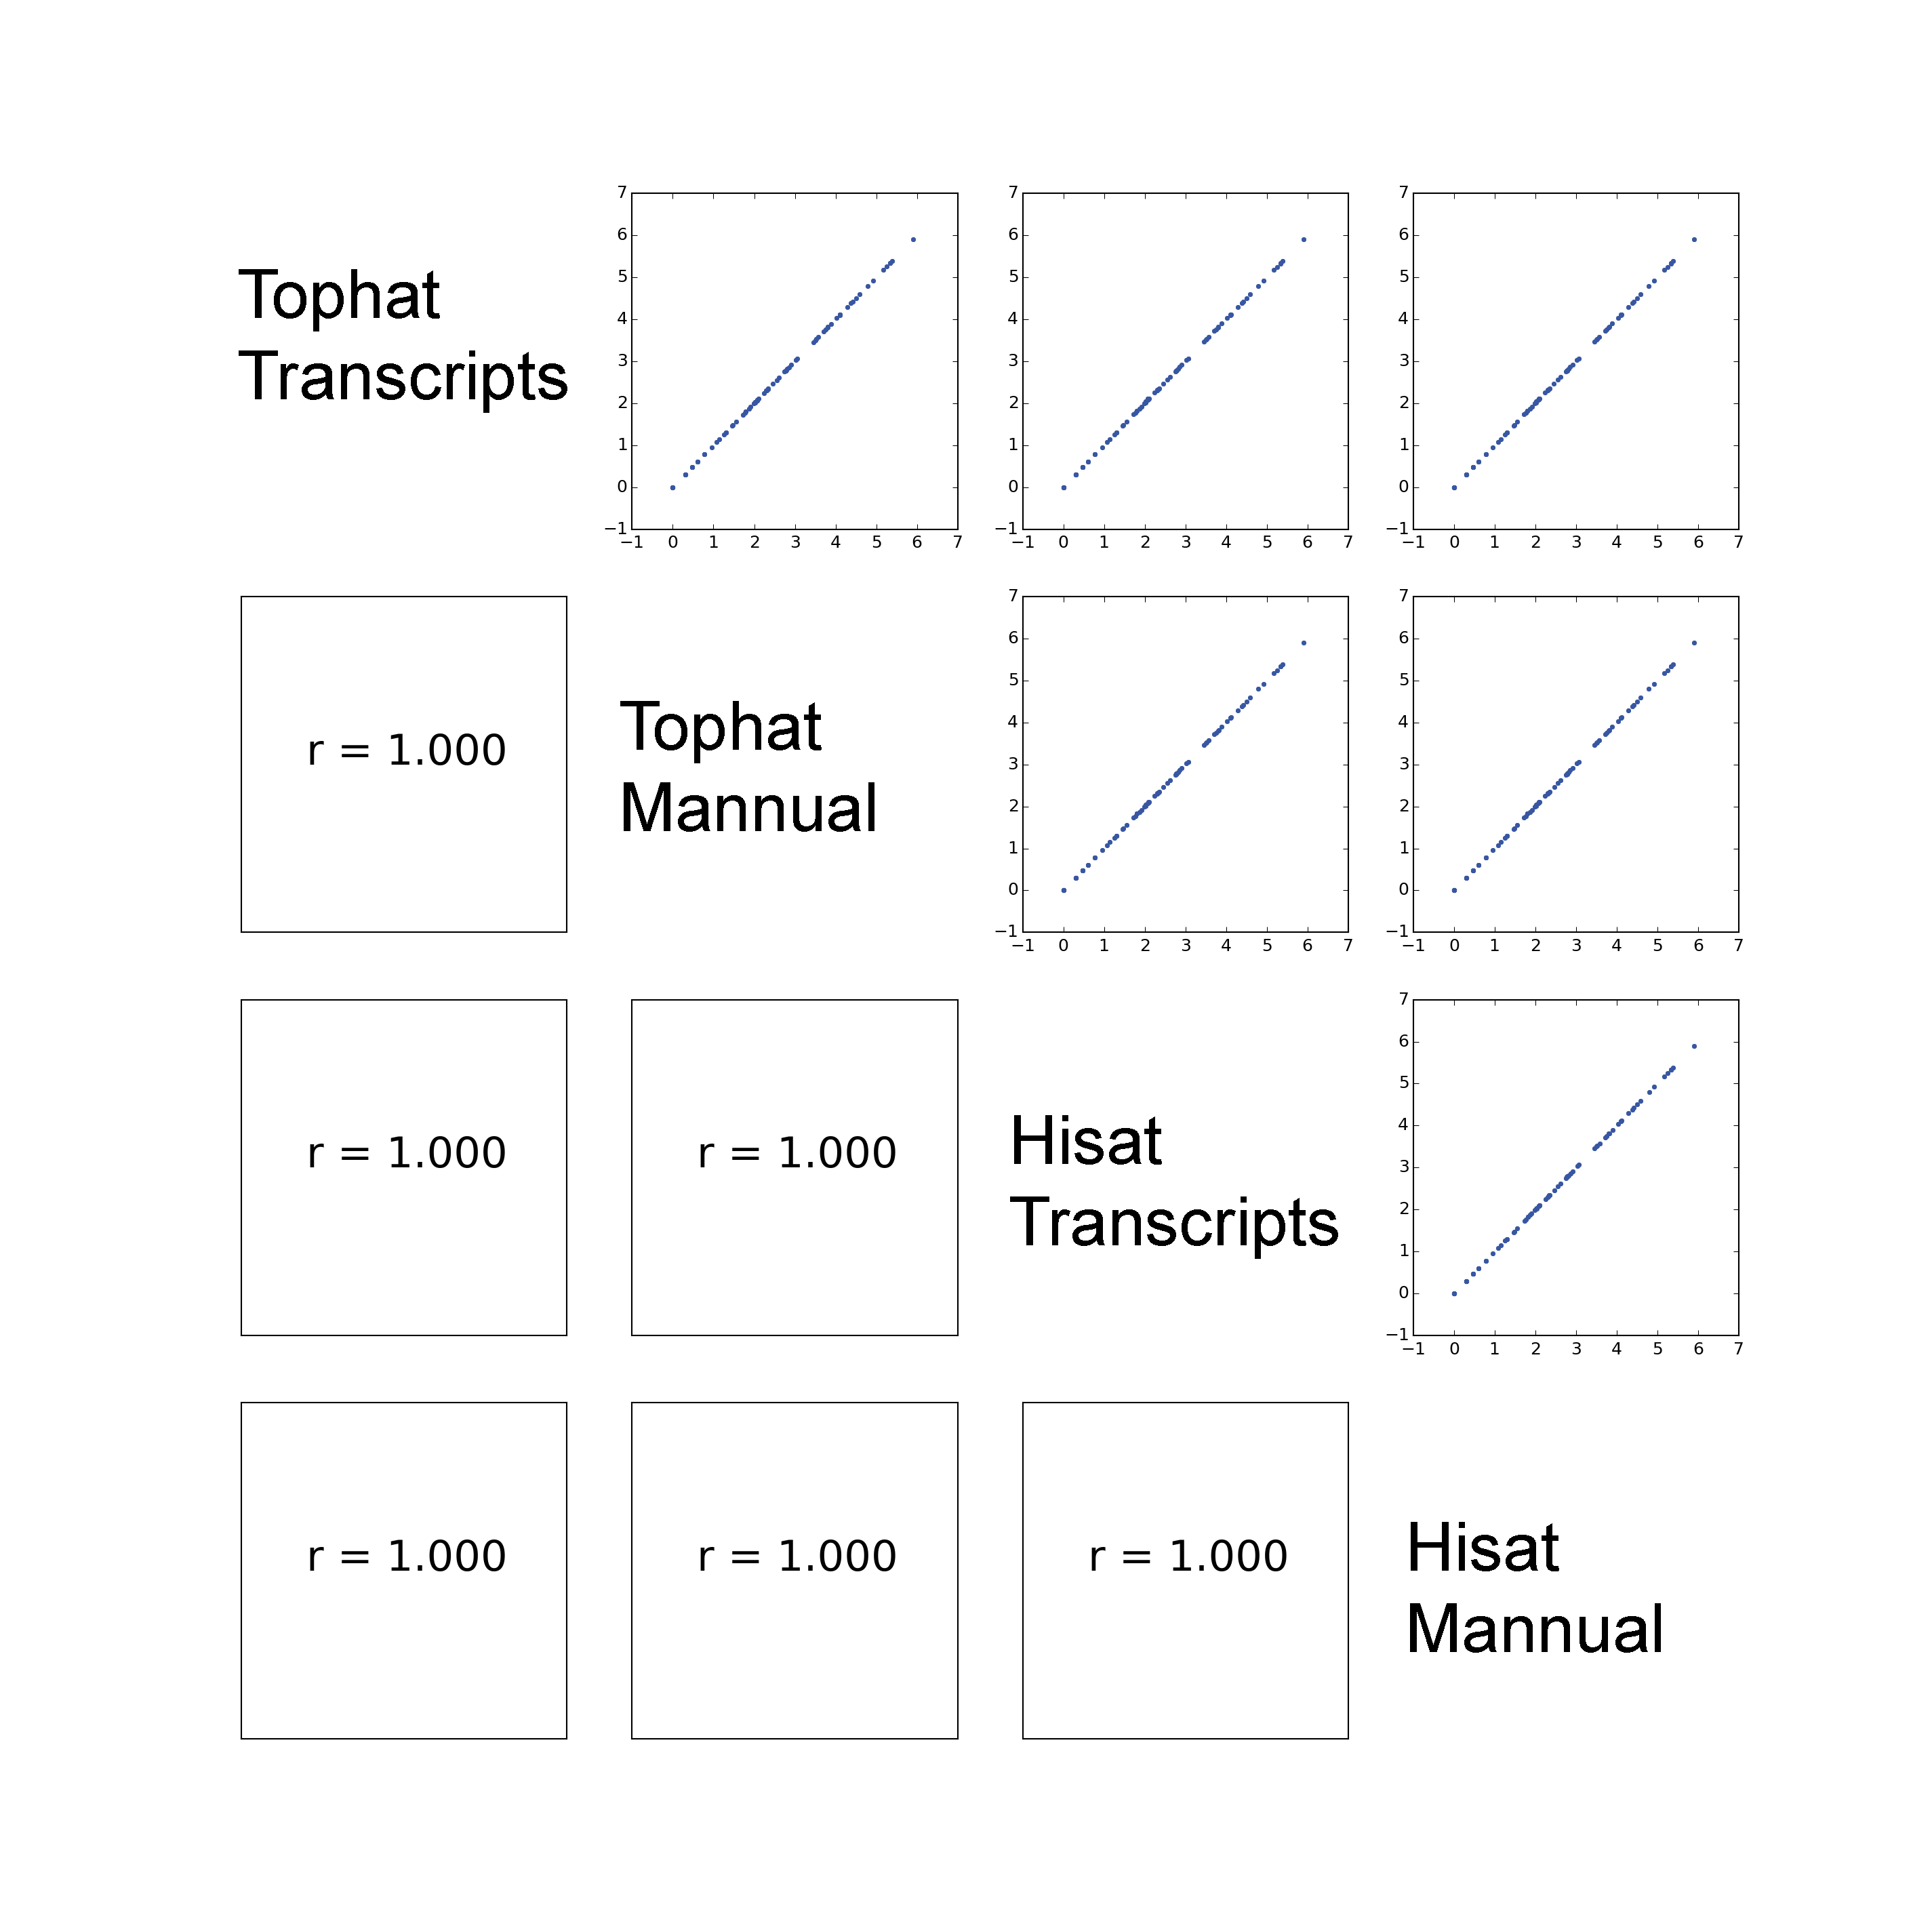
\includegraphics[height=4cm]{ERCC_count}	\\	
			\end{tabular}	
			\end{table}	
			\tiny{Why Hisat FPKM were higher but HTSeq unique count were almost the same? \\ \pause
			Hisat could find more multiple alignments. ERCC contained some repeat sequences.}
	\end{block}
\end{frame}


\begin{frame}[c,fragile]
	\frametitle{ Linc-RNA detection: TT $>$ TM $>$ HT = HM. }
	\begin{block}{ Read Counts for refseq-genes. }
			\begin{table}
			\centering	
			\begin{tabular}{C{3cm} C{3cm} C{3cm}}     
				Noncode 4.0		& nsmb 2660 & novo lincRNA 	\\
				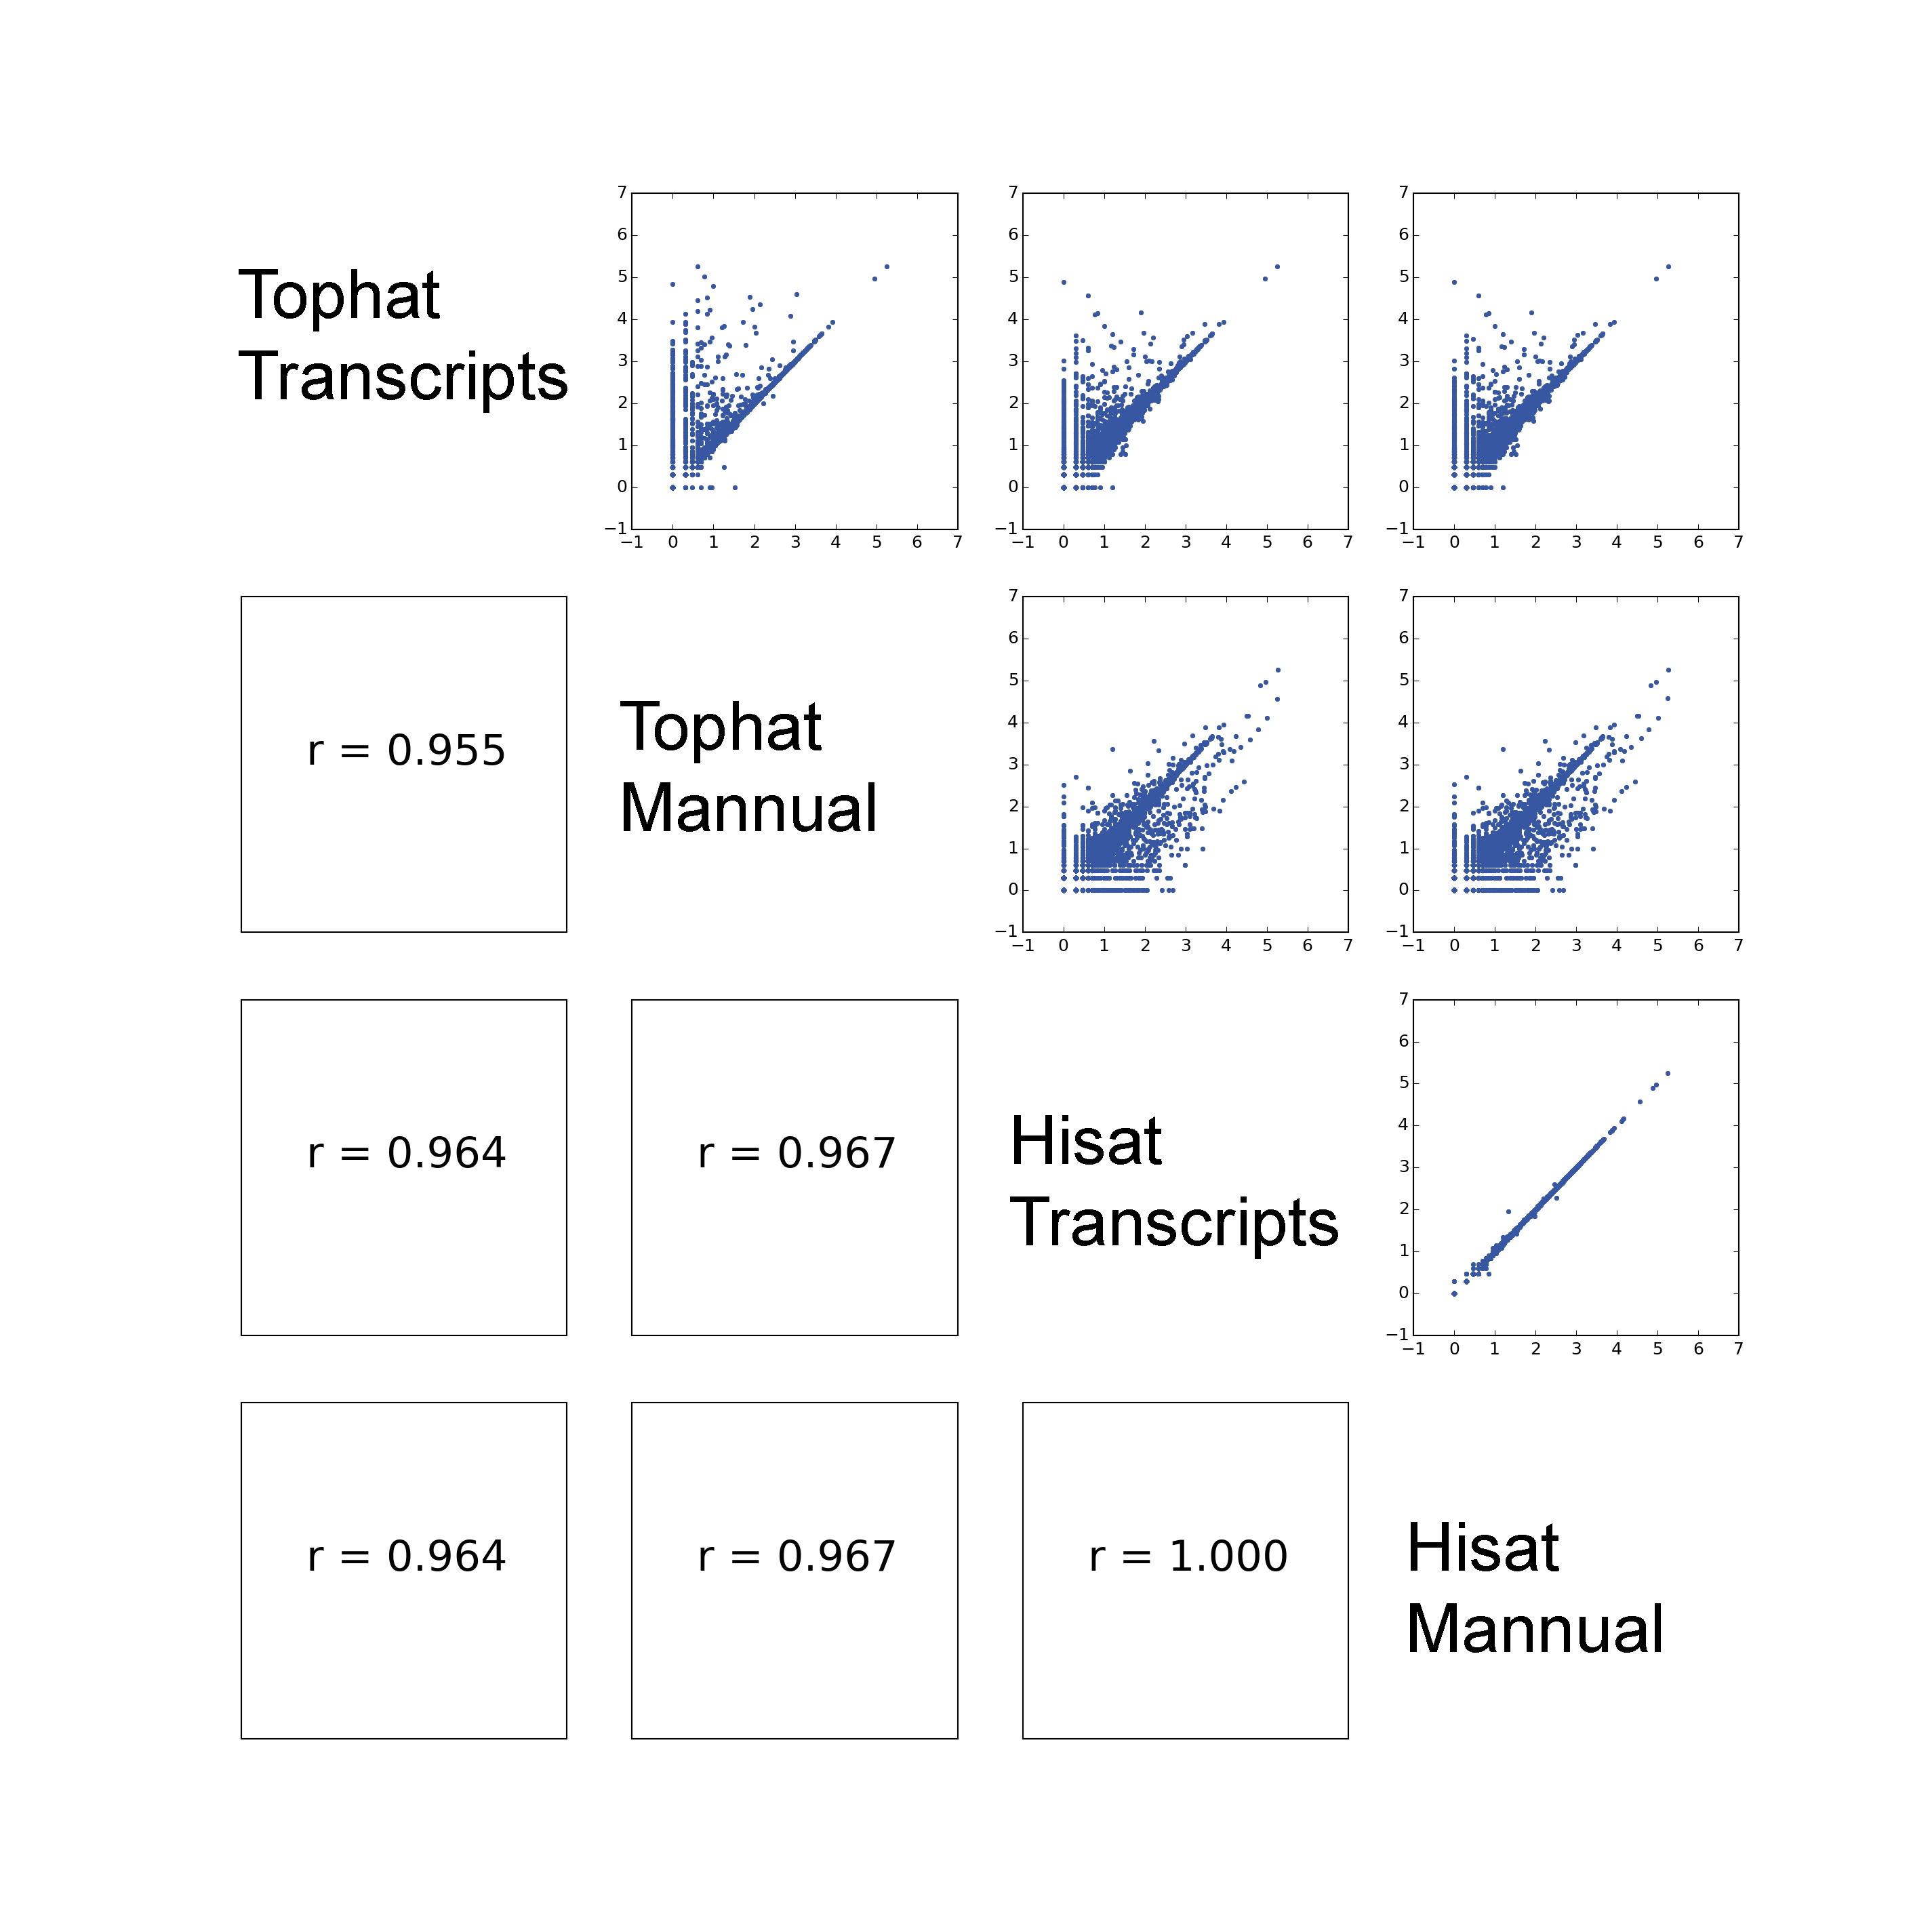
\includegraphics[height=3cm ]{Noncode_count} &  
				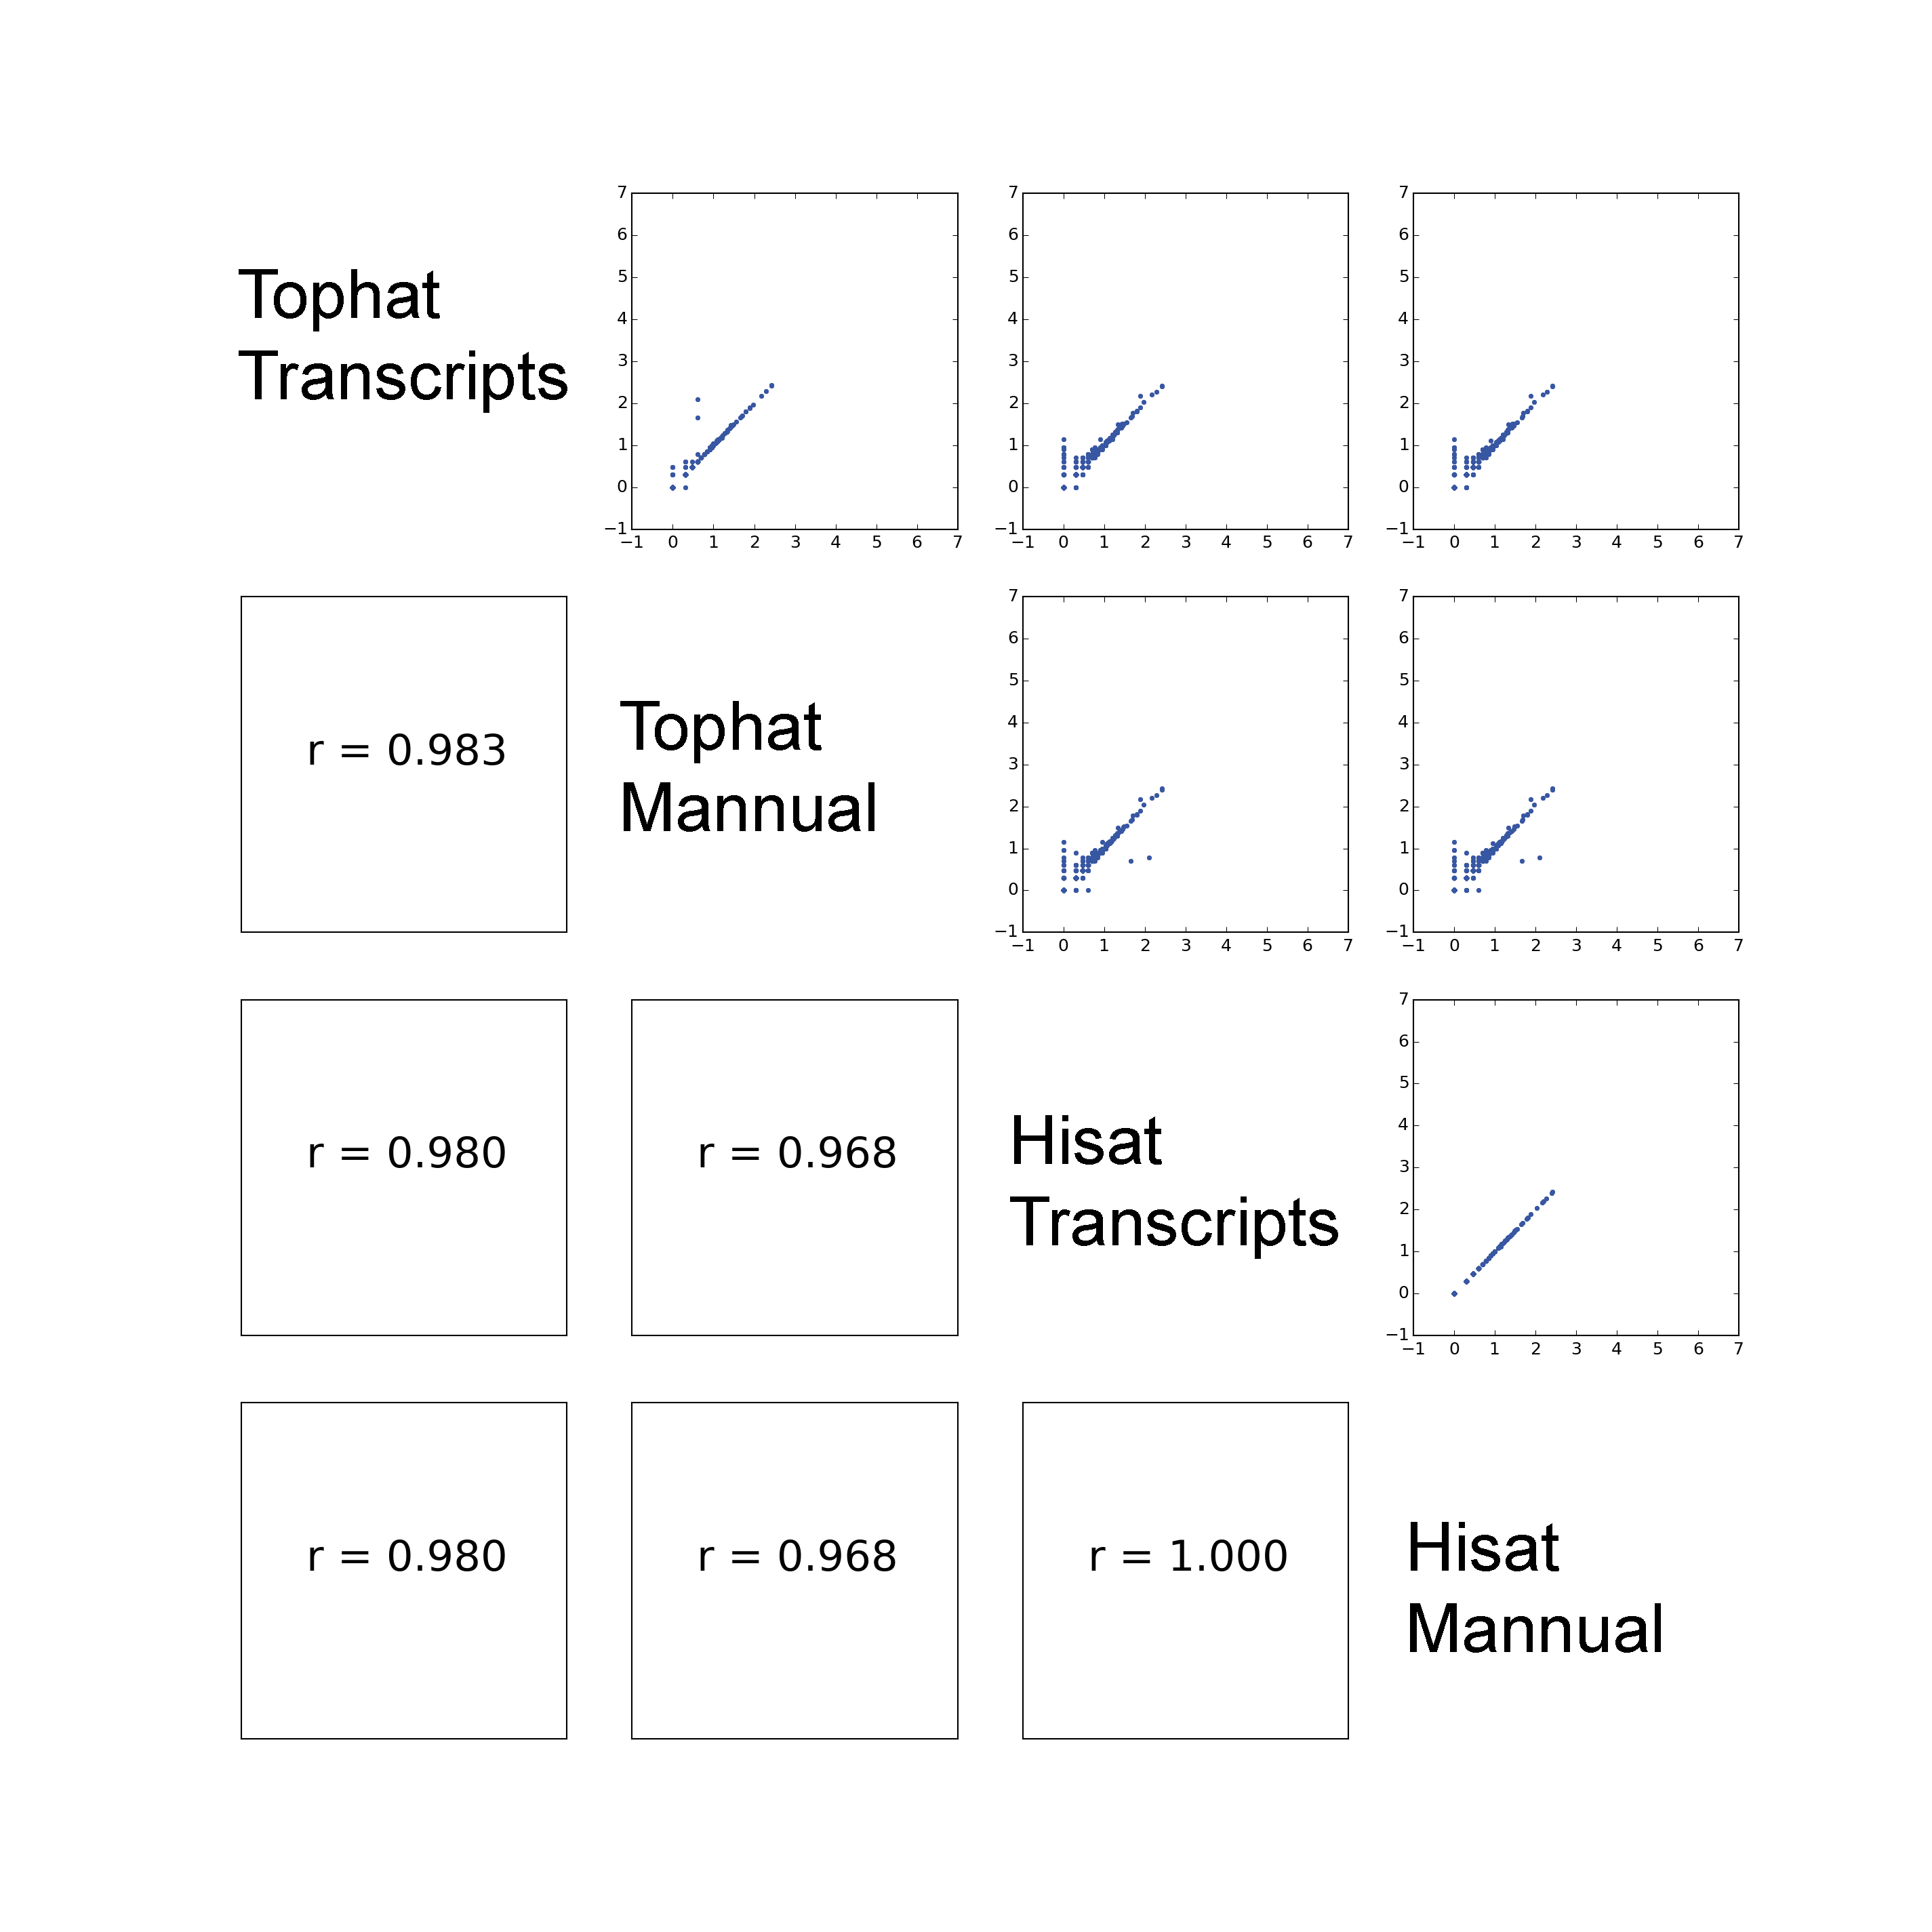
\includegraphics[height=3cm ]{NSMB_count}	 &
				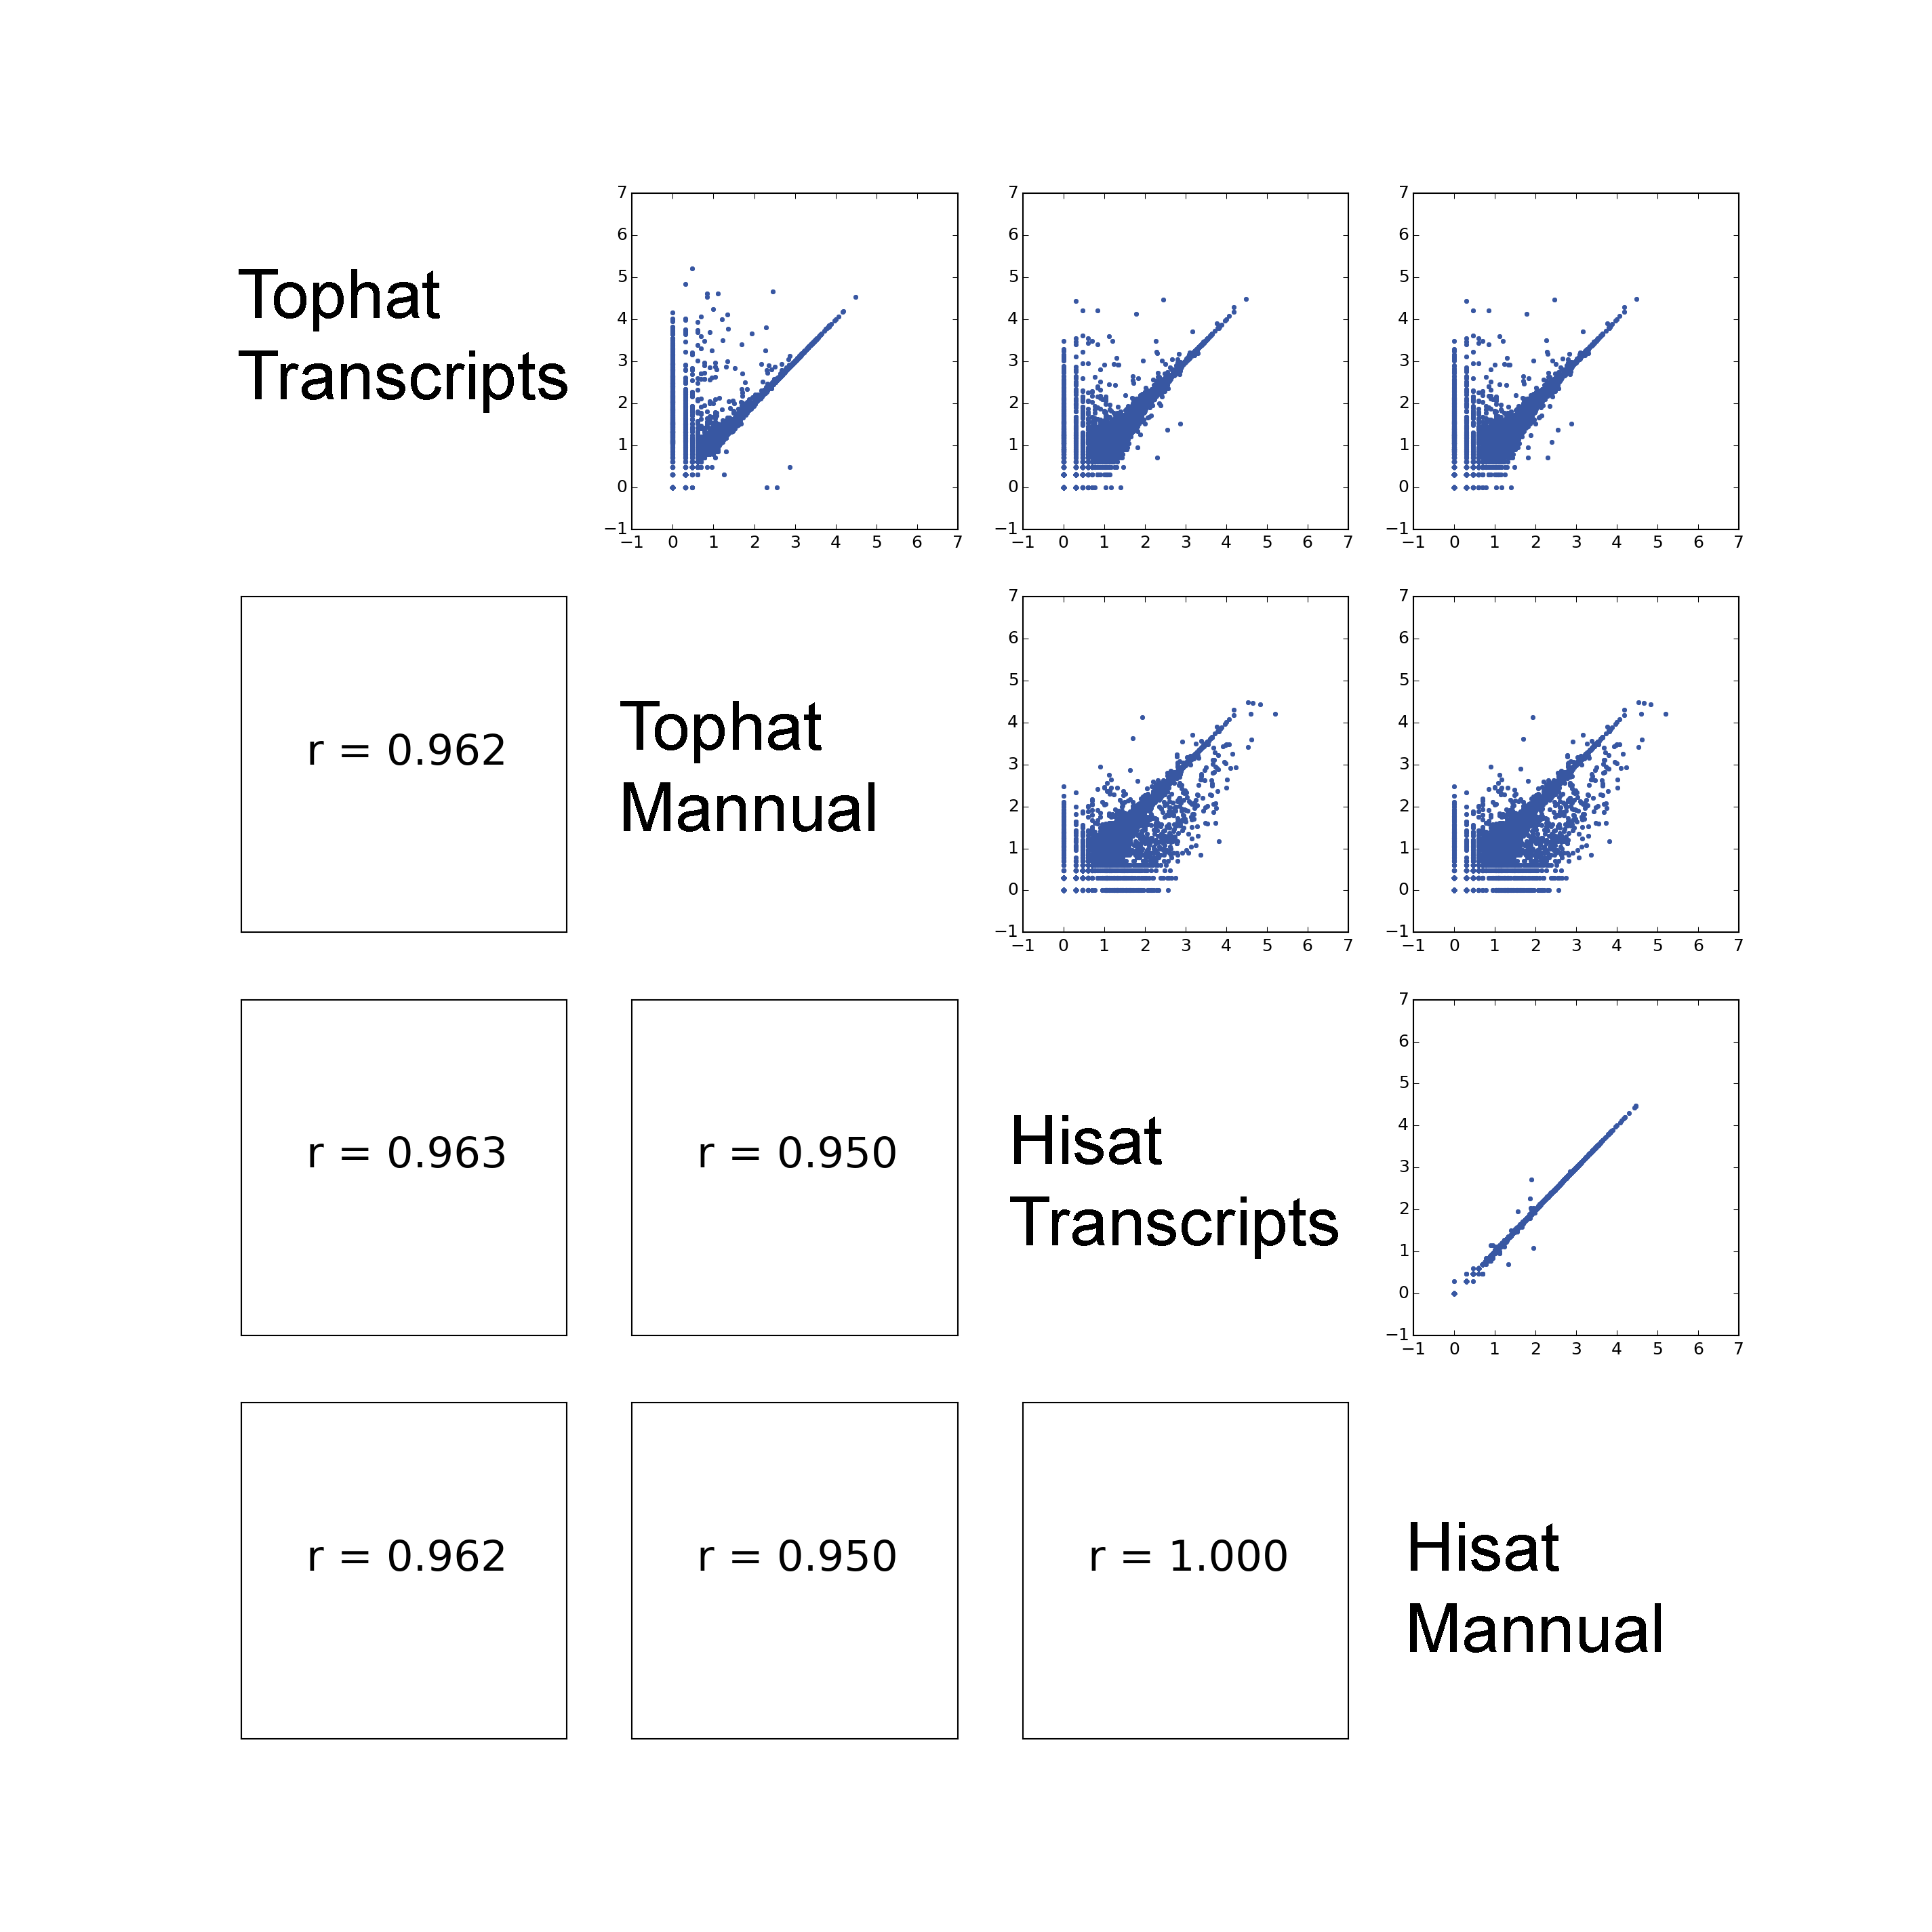
\includegraphics[height=3cm ]{Neo_count}	\\	
			\end{tabular}	
			\end{table}	
	\end{block}
\end{frame}



\subsection{3.Some case for different mapping.}

\begin{frame}[c,fragile]
	\frametitle{ Why some reads could only be mapped using Hisat. }
	\begin{block}{ case1. Hisat allows more mismatch.  }
		Tophat used \alert{"-N 2"} in the testing-script, which means the maxinum mismatch allowed in the given read. \\ \pause
		However, there were no such command for Hisat. \\ \pause
		If you require a maxinum mismatch for a successful mapping, just filter it by yourself using the resulting bam.
	\end{block}
\end{frame}

\begin{frame}[c,fragile]
	\begin{examples}
		$>$SRR534301.4\\
		\tiny{CGCCATCTGAGCCCTTCTCTTCAATCTCAGCCTTGAGGATCNNTAAGTCAGTAGTGAGCTCGTCCACCCGC\\TCCTNCNGNNCCTCCACCTCCTGCTGCAGG} \\
		\tiny{
			\begin{table}
			\centering
			\begin{tabular}{  C{1cm}  C{1.2cm}  C{1.2cm}  C{1.2cm}  C{1.2cm}  }
			\hline\noalign{\smallskip}
						& TT 	& HT  &	TM	 & HM  	\\
			\noalign{\smallskip}\hline\noalign{\smallskip}
			Chr:beg	&	-		& chr11:122928386   & - & chr11:122928386	\\
			Gene		&	-  	& HSPA8             & - & HSPA8          	\\
			\noalign{\smallskip}\hline 
			\end{tabular}
			\end{table}
		}
		\scriptsize{Tophat-Trans(TT) Hisat-Trans(HT) Tophat-Mannual(TM) Hisat2x-Mannual(HM).}
		\begin{lstlisting}[basicstyle=\tiny]
			
				SCORE START  END QSIZE IDENTITY CHRO STRAND  START    END      SPAN
				-------------------------------------------------------------------
				  94     1   101   101 100.0%     2   +   74597660  74597836    177
		
				00000063 tccacccgctcctncngnncctccacctcctgctgcagg 00000101
				>>>>>>>> ||||||||||||| | |  |||||||||||||||||||| >>>>>>>>
				74597798 tccacccgctccttcagtgcctccacctcctgctgcagg 74597836
		
		\end{lstlisting}
		\alert{3 mismatches}, above Tophat's cut-off(2).
		\end{examples}
	
\end{frame}

\begin{frame}[c,fragile]
	\frametitle{ Why some reads have different number of hits on genome. }
	\begin{block}{ case2. Pseudogenes.  }
		\begin{itemize}
			\item A read can both map to a protein-coding gene and a pseudogene. \\ \pause
			\item A junction for a protein-coding gene, and a mismatch for pseudogene. \\ \pause
			\item Junction is more realiable because of the existance of exons.	\\ \pause
			\item Penalty for mismatch is smaller.	\\ \pause
			\item Map reads to \alert{transcriptome first}.
		\end{itemize}
	\end{block}
\end{frame}

\begin{frame}[c,fragile]
	\begin{examples}
		$>$SRR534301.77\\
		\tiny{GTTGCTGGTGACAGCAAAAATGACCCACCAATGGAAGCAGCTGGCTTCACTGCTCAGGTGATTATCCTGAA\\CCATCCAGGCCAAATAAGCGCCGGCTATGC}
		\tiny{
			\begin{table}
			\centering
			\begin{tabular}{  C{1cm}  C{1.2cm}  C{1.2cm}  C{1.2cm}  C{1.2cm}  }
			\hline\noalign{\smallskip}
						& TT 	& HT  &	TM	 & HM  	\\
			\noalign{\smallskip}\hline\noalign{\smallskip}
			Chr:beg	&	chr6:74227944		& chr6:74227944 chr9:135895845    &	chr9:135895845 & chr6:74227944 chr9:135895845	\\
			Gene		&	EEF1A1            & \_\_too\_low\_aQual \_\_too\_low\_aQual &	\_\_no\_feature   & \_\_too\_low\_aQual \_\_too\_low\_aQual	\\
			\noalign{\smallskip}\hline
			\end{tabular}
			\end{table}
		}
		
		\scriptsize{Tophat-Trans(TT) Hisat-Trans(HT) Tophat-Mannual(TM) Hisat2x-Mannual(HM).}
		\begin{lstlisting}[basicstyle=\tiny]
			
				SCORE START  END QSIZE IDENTITY CHRO STRAND  START    END      SPAN
				-------------------------------------------------------------------
				101     1   101   101 100.0%     9   +  135895845 135895945    101
				100     1   101   101 100.0%     6   -   74227944  74228133    190

		\end{lstlisting}
		\end{examples}
	
\end{frame}

\begin{frame}[c,fragile]
	\frametitle{ Perfectly mapped on two sites, one protein-coding gene, one pseudo gene }
	\begin{examples}

		\begin{lstlisting}[basicstyle=\tiny]
			
				SCORE START  END QSIZE IDENTITY CHRO STRAND  START    END      SPAN
				-------------------------------------------------------------------
				101     1   101   101 100.0%     9   +  135895845 135895945    101
				100     1   101   101 100.0%     6   -   74227944  74228133    190
				
				chr6: EEF1A1, protein-coding gene with 90bp junction.
				00000051 tgctcag  == gtgattatcctgaaccatccaggccaaataagcgccggctatgc 00000101
				<<<<<<<< |||||||  == |||||||||||||||||||||||||||||||||||||||||||| <<<<<<<<
				74228083 tgctcag  == gtgattatcctgaaccatccaggccaaataagcgccggctatgc 74227944
				
				chr9: EEFAL3, pseudo gene with no junction.
				000000051 tgctcaggtgattatcctgaaccatccaggccaaataagcgccggctatg 000000100
				>>>>>>>>> |||||||||||||||||||||||||||||||||||||||||||||||||| >>>>>>>>>
				135895895 tgctcaggtgattatcctgaaccatccaggccaaataagcgccggctatg 135895944

		\end{lstlisting}
		\end{examples}
	
\end{frame}


\begin{frame}[c,fragile]
\frametitle{ Hisat reported a multiple hit while tophat thought it mapped uniquely to a protein coding gene. }
	\begin{examples}
		\tiny{
			\begin{table}
			\centering
			\begin{tabular}{  C{1cm}  C{1.2cm}  C{1.2cm}  C{1.2cm}  C{1.2cm}  }
			\hline\noalign{\smallskip}
						& TT 	& HT  &	TM	 & HM  	\\
			\noalign{\smallskip}\hline\noalign{\smallskip}
			Chr:beg	&	chr6:74227944		& chr6:74227944 chr9:135895845    &	chr9:135895845 & chr6:74227944 chr9:135895845	\\
			\noalign{\smallskip}\hline
			\end{tabular}
			\end{table}
		}
		\begin{lstlisting}[basicstyle=\tiny]
				chr6: EEF1A1, protein-coding gene with 90bp junction.
				00000051 tgctcag  == gtgattatcctgaaccatccaggccaaataagcgccggctatgc 00000101
				<<<<<<<< |||||||  == |||||||||||||||||||||||||||||||||||||||||||| <<<<<<<<
				74228083 tgctcag  == gtgattatcctgaaccatccaggccaaataagcgccggctatgc 74227944
				
				chr9: EEFAL3, pseudo gene with no junction.
				000000051 tgctcaggtgattatcctgaaccatccaggccaaataagcgccggctatg 000000100
				>>>>>>>>> |||||||||||||||||||||||||||||||||||||||||||||||||| >>>>>>>>>
				135895895 tgctcaggtgattatcctgaaccatccaggccaaataagcgccggctatg 135895944

		\end{lstlisting}
		\scriptsize{
			\begin{itemize}
				\item Transcripts-first mapping will consider protein-coding gene priorly. \\ \pause
				\item If not, it will consider pseudo gene priorly. \\ \pause
				\item Hisat reports all perfect-match sites.
			\end{itemize}
		}
		\end{examples}
	
\end{frame}

\subsection{4.Comparing with spike-in molecules.}

\begin{frame}[c,fragile]
	\frametitle{ Using relative total molecules. }
	\begin{block}{ ERCC spike-in detected. }
		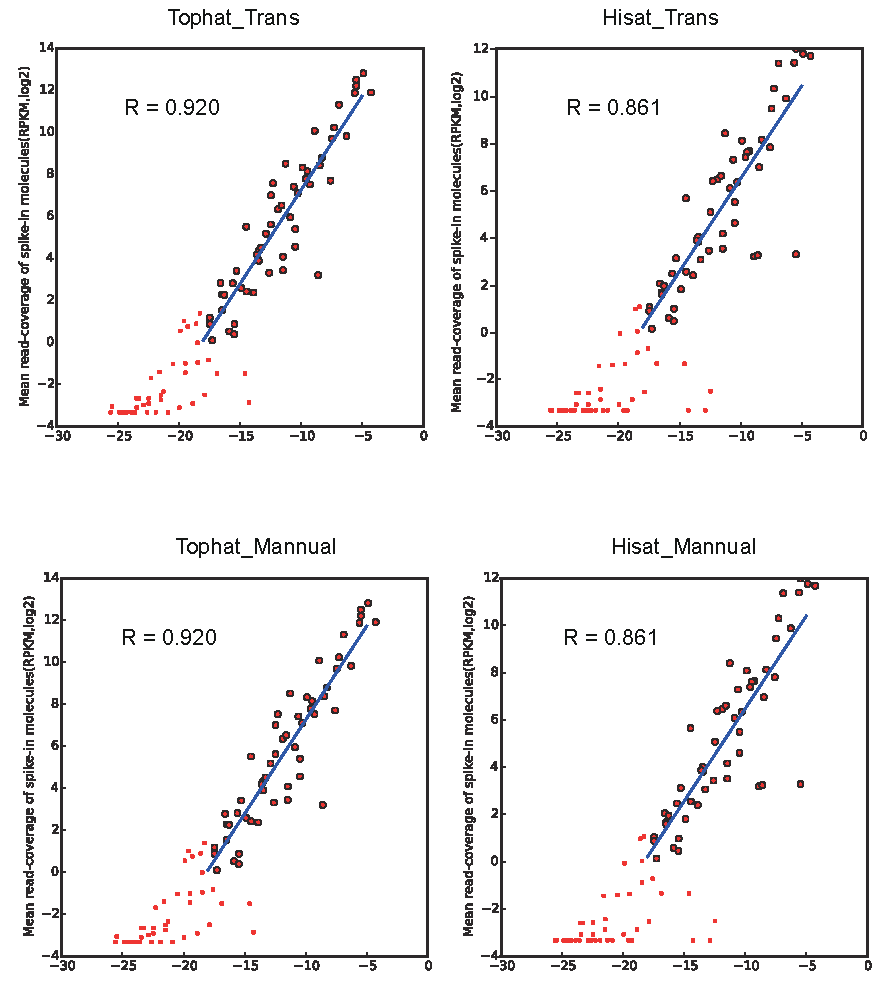
\includegraphics[height=5cm]{Ab_mol}
	\end{block}
\end{frame}

\subsection{5.Comparing with other methods.}
\begin{frame}[c,fragile]
	\frametitle{ Comparing RNA-seq with Taqman Gene Expression Assays. }
	\begin{block}{ Using method in nature07509, alternative isoform regulation in human tissue transcriptomes. }
		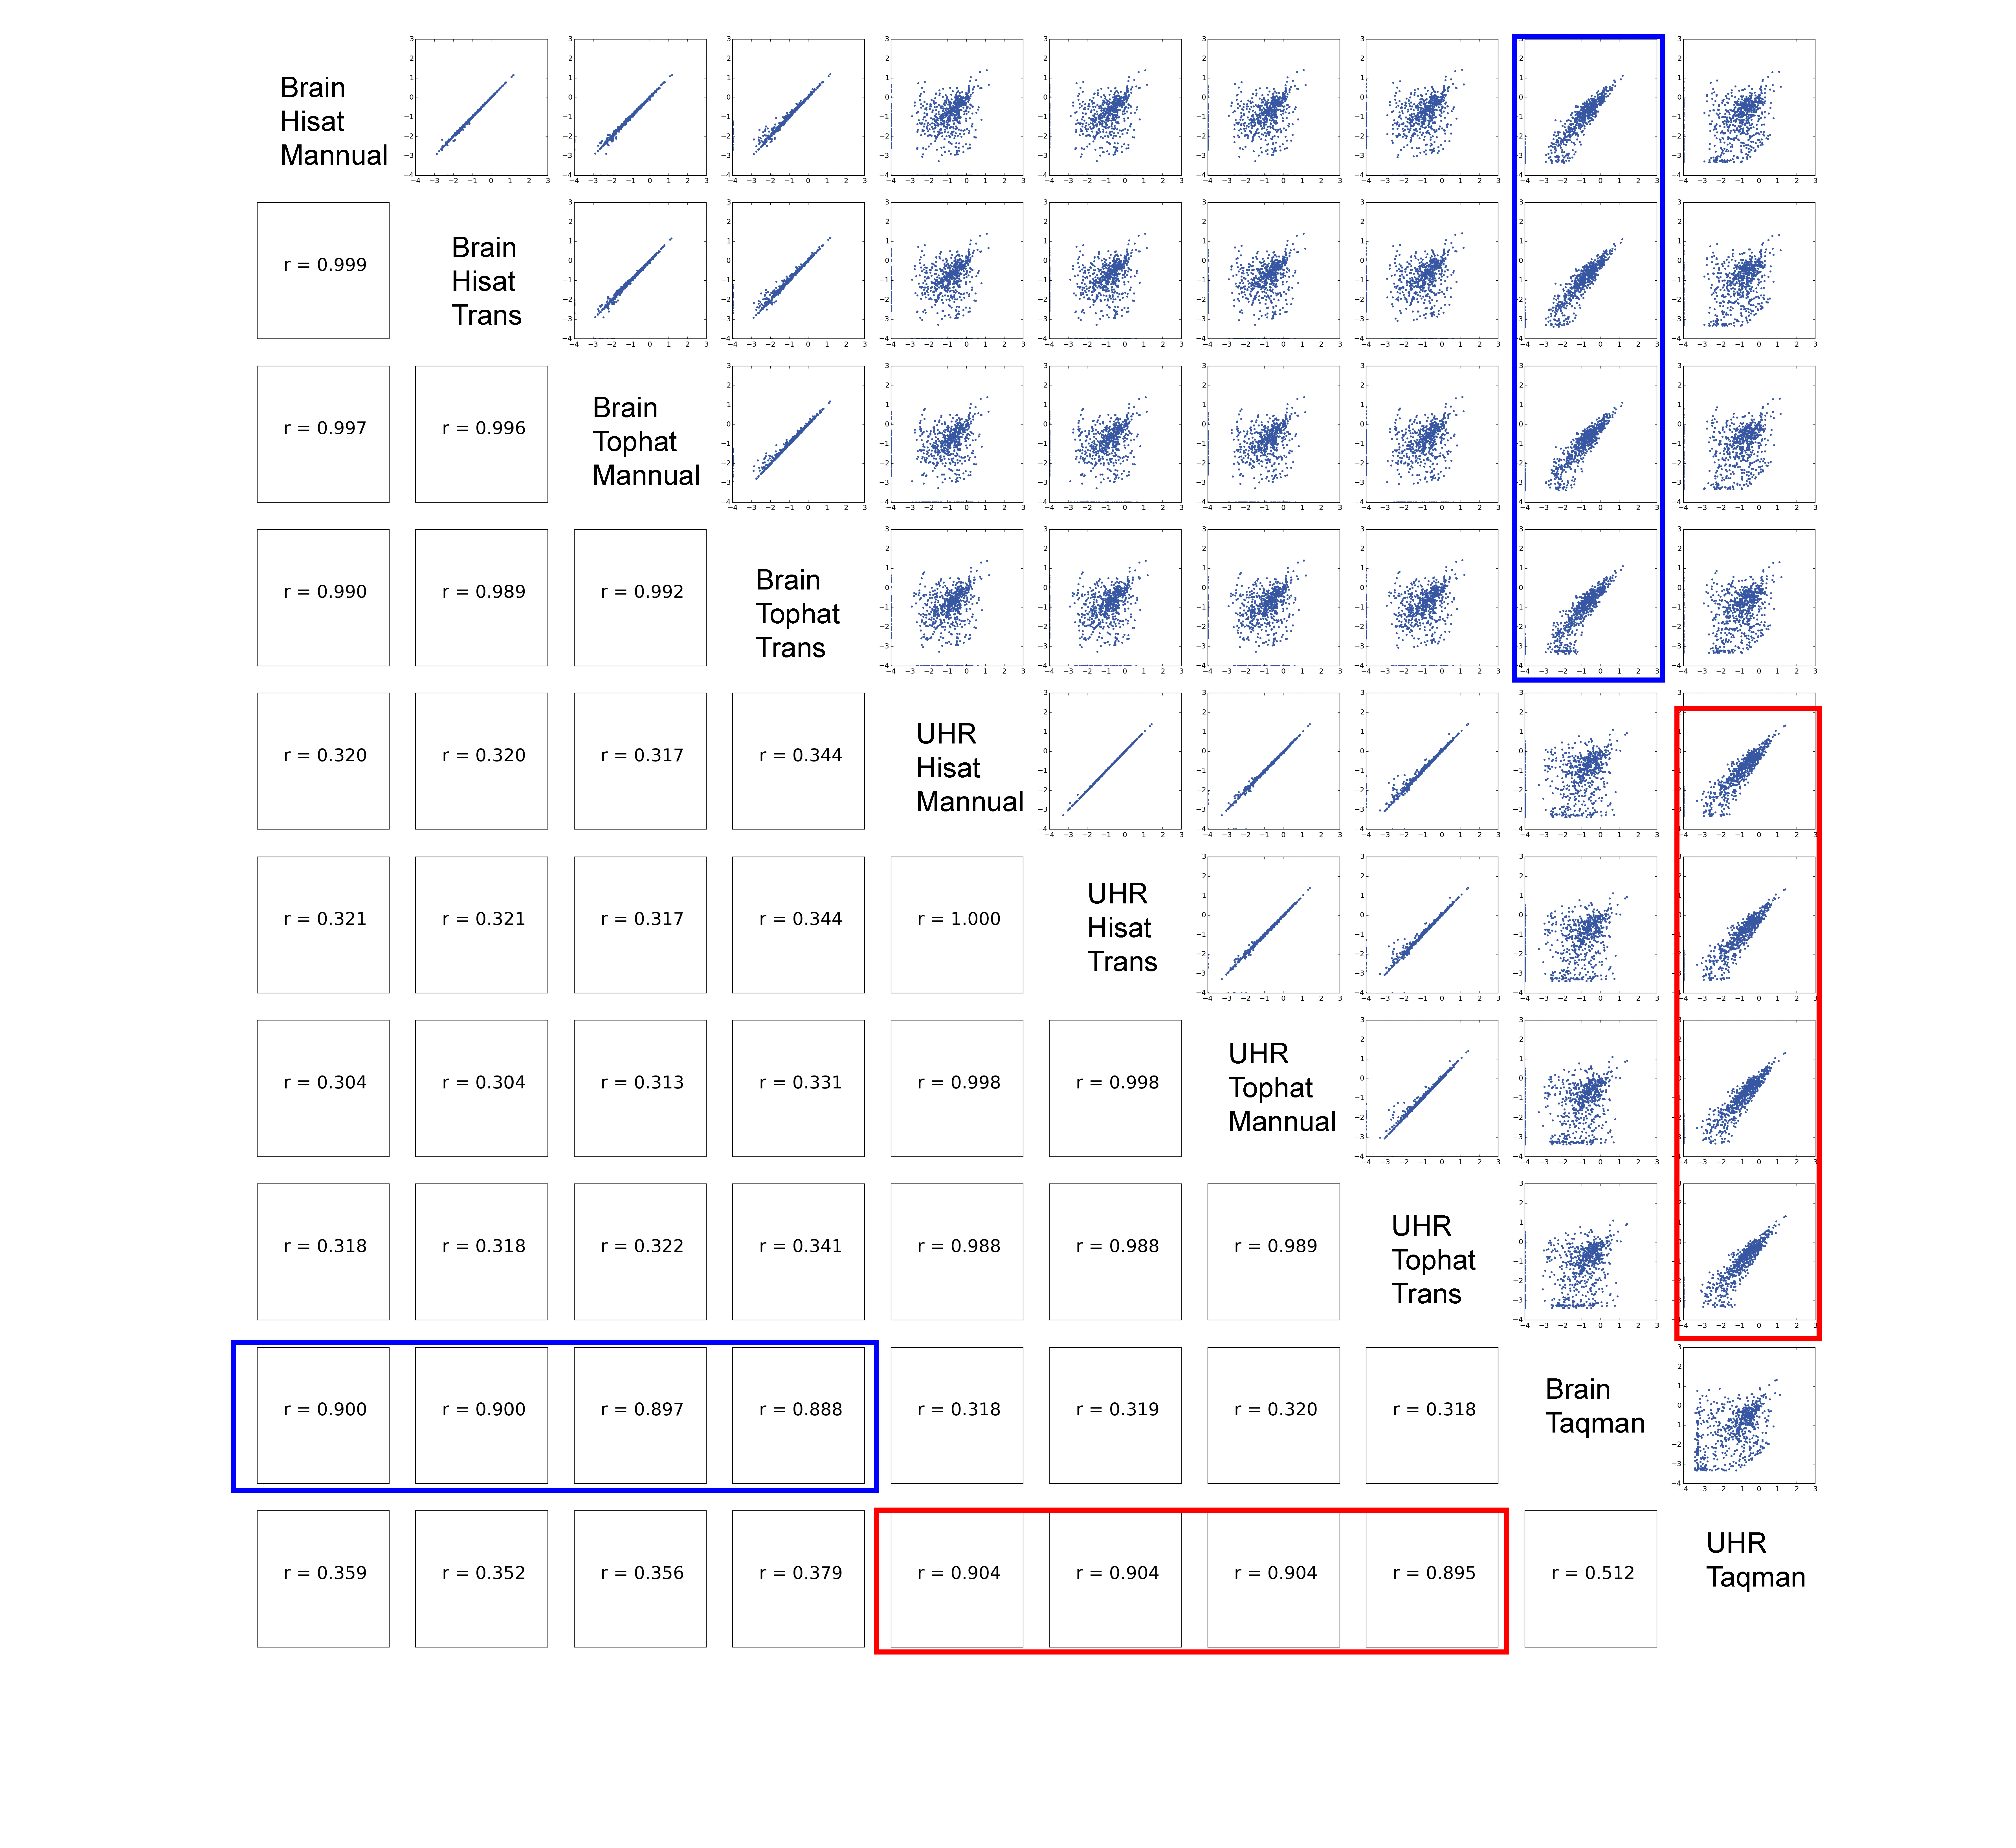
\includegraphics[height=5cm]{CompStandard}
	\end{block}
\end{frame}

\begin{frame}[c,fragile]
	\frametitle{ Comparing RNA-seq with Taqman Gene Expression Assays. }
	\begin{block}{ Result in nature07509. }
		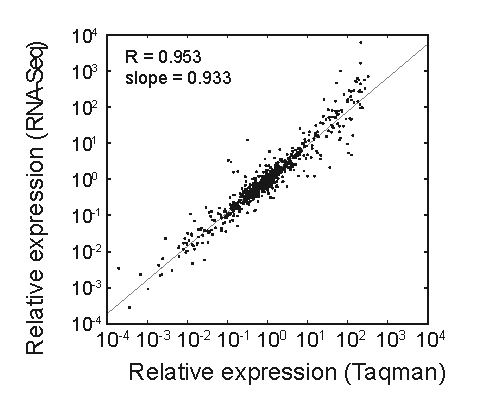
\includegraphics[height=5cm]{Standard_article}
	\end{block}
\end{frame}

\subsection{.}
